\documentclass{article}

\usepackage{arxiv}
\usepackage[utf8]{inputenc} % allow utf-8 input
\usepackage[T1]{fontenc}    % use 8-bit T1 fonts
\usepackage{hyperref}       % hyperlinks
\usepackage{url}            % simple URL typesetting
\usepackage{booktabs}       % professional-quality tables
\usepackage{amsfonts}       % blackboard math symbols
\usepackage{nicefrac}       % compact symbols for 1/2, etc.
\usepackage{microtype}      % microtypography
\usepackage{lipsum}		% Can be removed after putting your text content
\usepackage{graphicx}
%\usepackage{natbib}
\usepackage{doi}

%\addbibresource{references.bib} %Imports bibliography file

\usepackage{caption}
\usepackage{subcaption}
\usepackage{algpseudocode}
\usepackage{algorithm}
\usepackage{listings}
\usepackage{amsmath}
\usepackage{xcolor}
\usepackage{listings}

\lstdefinestyle{customc}{
    language=C,                      % Set language
    basicstyle=\small\ttfamily,       % Monospace font, small size
    keywordstyle=\color{blue},        % Keywords in blue
    commentstyle=\color{gray},        % Comments in gray
    stringstyle=\color{red},          % Strings in red
    numbers=left,                     % Line numbers on the left
    numberstyle=\tiny\color{gray},    % Line number style
    backgroundcolor=\color{lightgray!20}, % Light gray background
    frame=single,                     % Add a frame around the code
    tabsize=4,                        % Set tab size
    breaklines=true                    % Enable line breaking
}

\lstset{style=customc}  % Apply the style globally


\newcommand{\frameworkName}{VIC } 

\title{VIC: Evasive Video Game Cheating via Virtual Machine Introspection}

%\date{September 9, 1985}	% Here you can change the date presented in the paper title
%\date{} 					% Or removing it

\author{ \href{https://orcid.org/0000-0002-3110-019X}{\includegraphics[scale=0.06]{orcid.pdf}\hspace{1mm}Panicos Karkallis} \\
	Royal Holloway University of London\\
	Egham, United Kingdom \\
	\texttt{panicos.karkallis.2018@rhul.ac.uk} \\
	%% examples of more authors
	\And
	\href{https://orcid.org/0000-0003-4392-9023}{\includegraphics[scale=0.06]{orcid.pdf}\hspace{1mm}Jorge Blasco Alís} \\
        Computer Systems Department \\
	Universidad Politécnica de Madrid\\
	Madrid, Spain \\
	\texttt{jorge.blasco.alis@upm.es} \\
	%% \AND
	%% Coauthor \\
	%% Affiliation \\
	%% Address \\
	%% \texttt{email} \\
	%% \And
	%% Coauthor \\
	%% Affiliation \\
	%% Address \\
	%% \texttt{email} \\
	%% \And
	%% Coauthor \\
	%% Affiliation \\
	%% Address \\
	%% \texttt{email} \\
}

% Uncomment to remove the date
%\date{}

% Uncomment to override  the `A preprint' in the header
%\renewcommand{\headeright}{Technical Report}
%\renewcommand{\undertitle}{Technical Report}
\renewcommand{\shorttitle}{\textit{VIC} Virtual Machine Introspection Cheat }

%%% Add PDF metadata to help others organize their library
%%% Once the PDF is generated, you can check the metadata with
%%% $ pdfinfo template.pdf
\hypersetup{
pdftitle={VIC - Evasive Video Game Cheating via Virtual Machine Introspection},
pdfsubject={q-bio.NC, q-bio.QM},
pdfauthor={Panicos Karkallis, Jorge Blasco Alis},
pdfkeywords={Online video game hacking, video game security, virtual machine introspection},
}

\begin{document}
\maketitle

\begin{abstract}
	Video game cheats modify a video game behaviour to give unfair advantages to some players while bypassing the methods game developers use to detect them. This destroys the experience of online gaming and can result in financial loses for game developers. In this work, we present a new type of game cheat, Virtual machine Introspection Cheats (VIC), that takes advantage of virtual machines to stealthy execute game cheats. \frameworkName employees a hypervisor with introspection enabled to lower down the bar of cheating against legacy and modern anti-cheat systems. We demonstrate the feasibility and stealthiness of \frameworkName against three popular games (Fortnite, BlackSquad and Team Fortress 2) that together include five different anti-cheats. In particular, we use \frameworkName to implement a cheat radar, a wall-hack cheat and a trigger-bot. To support our claim that this type of cheats can be effectively used, we present the performance impact that \frameworkName has on gameplay by monitoring the frames per second (fps) while the cheats are activated. Our experimentation also shows how these cheats are currently undetected by the most popular anti-cheat systems, enabling a new paradigm that can take advantage of cloud infrastructure to offer cheating-as-a-service.
\end{abstract}


% keywords can be removed
\keywords{Online video game hacking, video game security, virtual machine introspection}
\textbf{\textit{ACM-Class: }}D.4.6

\section{Introduction}
\label{sec:introduction}
The business processes of organizations are experiencing ever-increasing complexity due to the large amount of data, high number of users, and high-tech devices involved \cite{martin2021pmopportunitieschallenges, beerepoot2023biggestbpmproblems}. This complexity may cause business processes to deviate from normal control flow due to unforeseen and disruptive anomalies \cite{adams2023proceddsriftdetection}. These control-flow anomalies manifest as unknown, skipped, and wrongly-ordered activities in the traces of event logs monitored from the execution of business processes \cite{ko2023adsystematicreview}. For the sake of clarity, let us consider an illustrative example of such anomalies. Figure \ref{FP_ANOMALIES} shows a so-called event log footprint, which captures the control flow relations of four activities of a hypothetical event log. In particular, this footprint captures the control-flow relations between activities \texttt{a}, \texttt{b}, \texttt{c} and \texttt{d}. These are the causal ($\rightarrow$) relation, concurrent ($\parallel$) relation, and other ($\#$) relations such as exclusivity or non-local dependency \cite{aalst2022pmhandbook}. In addition, on the right are six traces, of which five exhibit skipped, wrongly-ordered and unknown control-flow anomalies. For example, $\langle$\texttt{a b d}$\rangle$ has a skipped activity, which is \texttt{c}. Because of this skipped activity, the control-flow relation \texttt{b}$\,\#\,$\texttt{d} is violated, since \texttt{d} directly follows \texttt{b} in the anomalous trace.
\begin{figure}[!t]
\centering
\includegraphics[width=0.9\columnwidth]{images/FP_ANOMALIES.png}
\caption{An example event log footprint with six traces, of which five exhibit control-flow anomalies.}
\label{FP_ANOMALIES}
\end{figure}

\subsection{Control-flow anomaly detection}
Control-flow anomaly detection techniques aim to characterize the normal control flow from event logs and verify whether these deviations occur in new event logs \cite{ko2023adsystematicreview}. To develop control-flow anomaly detection techniques, \revision{process mining} has seen widespread adoption owing to process discovery and \revision{conformance checking}. On the one hand, process discovery is a set of algorithms that encode control-flow relations as a set of model elements and constraints according to a given modeling formalism \cite{aalst2022pmhandbook}; hereafter, we refer to the Petri net, a widespread modeling formalism. On the other hand, \revision{conformance checking} is an explainable set of algorithms that allows linking any deviations with the reference Petri net and providing the fitness measure, namely a measure of how much the Petri net fits the new event log \cite{aalst2022pmhandbook}. Many control-flow anomaly detection techniques based on \revision{conformance checking} (hereafter, \revision{conformance checking}-based techniques) use the fitness measure to determine whether an event log is anomalous \cite{bezerra2009pmad, bezerra2013adlogspais, myers2018icsadpm, pecchia2020applicationfailuresanalysispm}. 

The scientific literature also includes many \revision{conformance checking}-independent techniques for control-flow anomaly detection that combine specific types of trace encodings with machine/deep learning \cite{ko2023adsystematicreview, tavares2023pmtraceencoding}. Whereas these techniques are very effective, their explainability is challenging due to both the type of trace encoding employed and the machine/deep learning model used \cite{rawal2022trustworthyaiadvances,li2023explainablead}. Hence, in the following, we focus on the shortcomings of \revision{conformance checking}-based techniques to investigate whether it is possible to support the development of competitive control-flow anomaly detection techniques while maintaining the explainable nature of \revision{conformance checking}.
\begin{figure}[!t]
\centering
\includegraphics[width=\columnwidth]{images/HIGH_LEVEL_VIEW.png}
\caption{A high-level view of the proposed framework for combining \revision{process mining}-based feature extraction with dimensionality reduction for control-flow anomaly detection.}
\label{HIGH_LEVEL_VIEW}
\end{figure}

\subsection{Shortcomings of \revision{conformance checking}-based techniques}
Unfortunately, the detection effectiveness of \revision{conformance checking}-based techniques is affected by noisy data and low-quality Petri nets, which may be due to human errors in the modeling process or representational bias of process discovery algorithms \cite{bezerra2013adlogspais, pecchia2020applicationfailuresanalysispm, aalst2016pm}. Specifically, on the one hand, noisy data may introduce infrequent and deceptive control-flow relations that may result in inconsistent fitness measures, whereas, on the other hand, checking event logs against a low-quality Petri net could lead to an unreliable distribution of fitness measures. Nonetheless, such Petri nets can still be used as references to obtain insightful information for \revision{process mining}-based feature extraction, supporting the development of competitive and explainable \revision{conformance checking}-based techniques for control-flow anomaly detection despite the problems above. For example, a few works outline that token-based \revision{conformance checking} can be used for \revision{process mining}-based feature extraction to build tabular data and develop effective \revision{conformance checking}-based techniques for control-flow anomaly detection \cite{singh2022lapmsh, debenedictis2023dtadiiot}. However, to the best of our knowledge, the scientific literature lacks a structured proposal for \revision{process mining}-based feature extraction using the state-of-the-art \revision{conformance checking} variant, namely alignment-based \revision{conformance checking}.

\subsection{Contributions}
We propose a novel \revision{process mining}-based feature extraction approach with alignment-based \revision{conformance checking}. This variant aligns the deviating control flow with a reference Petri net; the resulting alignment can be inspected to extract additional statistics such as the number of times a given activity caused mismatches \cite{aalst2022pmhandbook}. We integrate this approach into a flexible and explainable framework for developing techniques for control-flow anomaly detection. The framework combines \revision{process mining}-based feature extraction and dimensionality reduction to handle high-dimensional feature sets, achieve detection effectiveness, and support explainability. Notably, in addition to our proposed \revision{process mining}-based feature extraction approach, the framework allows employing other approaches, enabling a fair comparison of multiple \revision{conformance checking}-based and \revision{conformance checking}-independent techniques for control-flow anomaly detection. Figure \ref{HIGH_LEVEL_VIEW} shows a high-level view of the framework. Business processes are monitored, and event logs obtained from the database of information systems. Subsequently, \revision{process mining}-based feature extraction is applied to these event logs and tabular data input to dimensionality reduction to identify control-flow anomalies. We apply several \revision{conformance checking}-based and \revision{conformance checking}-independent framework techniques to publicly available datasets, simulated data of a case study from railways, and real-world data of a case study from healthcare. We show that the framework techniques implementing our approach outperform the baseline \revision{conformance checking}-based techniques while maintaining the explainable nature of \revision{conformance checking}.

In summary, the contributions of this paper are as follows.
\begin{itemize}
    \item{
        A novel \revision{process mining}-based feature extraction approach to support the development of competitive and explainable \revision{conformance checking}-based techniques for control-flow anomaly detection.
    }
    \item{
        A flexible and explainable framework for developing techniques for control-flow anomaly detection using \revision{process mining}-based feature extraction and dimensionality reduction.
    }
    \item{
        Application to synthetic and real-world datasets of several \revision{conformance checking}-based and \revision{conformance checking}-independent framework techniques, evaluating their detection effectiveness and explainability.
    }
\end{itemize}

The rest of the paper is organized as follows.
\begin{itemize}
    \item Section \ref{sec:related_work} reviews the existing techniques for control-flow anomaly detection, categorizing them into \revision{conformance checking}-based and \revision{conformance checking}-independent techniques.
    \item Section \ref{sec:abccfe} provides the preliminaries of \revision{process mining} to establish the notation used throughout the paper, and delves into the details of the proposed \revision{process mining}-based feature extraction approach with alignment-based \revision{conformance checking}.
    \item Section \ref{sec:framework} describes the framework for developing \revision{conformance checking}-based and \revision{conformance checking}-independent techniques for control-flow anomaly detection that combine \revision{process mining}-based feature extraction and dimensionality reduction.
    \item Section \ref{sec:evaluation} presents the experiments conducted with multiple framework and baseline techniques using data from publicly available datasets and case studies.
    \item Section \ref{sec:conclusions} draws the conclusions and presents future work.
\end{itemize}
\section{Background}\label{sec:backgrnd}

\subsection{Cold Start Latency and Mitigation Techniques}

Traditional FaaS platforms mitigate cold starts through snapshotting, lightweight virtualization, and warm-state management. Snapshot-based methods like \textbf{REAP} and \textbf{Catalyzer} reduce initialization time by preloading or restoring container states but require significant memory and I/O resources, limiting scalability~\cite{dong_catalyzer_2020, ustiugov_benchmarking_2021}. Lightweight virtualization solutions, such as \textbf{Firecracker} microVMs, achieve fast startup times with strong isolation but depend on robust infrastructure, making them less adaptable to fluctuating workloads~\cite{agache_firecracker_2020}. Warm-state management techniques like \textbf{Faa\$T}~\cite{romero_faa_2021} and \textbf{Kraken}~\cite{vivek_kraken_2021} keep frequently invoked containers ready, balancing readiness and cost efficiency under predictable workloads but incurring overhead when demand is erratic~\cite{romero_faa_2021, vivek_kraken_2021}. While these methods perform well in resource-rich cloud environments, their resource intensity challenges applicability in edge settings.

\subsubsection{Edge FaaS Perspective}

In edge environments, cold start mitigation emphasizes lightweight designs, resource sharing, and hybrid task distribution. Lightweight execution environments like unikernels~\cite{edward_sock_2018} and \textbf{Firecracker}~\cite{agache_firecracker_2020}, as used by \textbf{TinyFaaS}~\cite{pfandzelter_tinyfaas_2020}, minimize resource usage and initialization delays but require careful orchestration to avoid resource contention. Function co-location, demonstrated by \textbf{Photons}~\cite{v_dukic_photons_2020}, reduces redundant initializations by sharing runtime resources among related functions, though this complicates isolation in multi-tenant setups~\cite{v_dukic_photons_2020}. Hybrid offloading frameworks like \textbf{GeoFaaS}~\cite{malekabbasi_geofaas_2024} balance edge-cloud workloads by offloading latency-tolerant tasks to the cloud and reserving edge resources for real-time operations, requiring reliable connectivity and efficient task management. These edge-specific strategies address cold starts effectively but introduce challenges in scalability and orchestration.

\subsection{Predictive Scaling and Caching Techniques}

Efficient resource allocation is vital for maintaining low latency and high availability in serverless platforms. Predictive scaling and caching techniques dynamically provision resources and reduce cold start latency by leveraging workload prediction and state retention.
Traditional FaaS platforms use predictive scaling and caching to optimize resources, employing techniques (OFC, FaasCache) to reduce cold starts. However, these methods rely on centralized orchestration and workload predictability, limiting their effectiveness in dynamic, resource-constrained edge environments.



\subsubsection{Edge FaaS Perspective}

Edge FaaS platforms adapt predictive scaling and caching techniques to constrain resources and heterogeneous environments. \textbf{EDGE-Cache}~\cite{kim_delay-aware_2022} uses traffic profiling to selectively retain high-priority functions, reducing memory overhead while maintaining readiness for frequent requests. Hybrid frameworks like \textbf{GeoFaaS}~\cite{malekabbasi_geofaas_2024} implement distributed caching to balance resources between edge and cloud nodes, enabling low-latency processing for critical tasks while offloading less critical workloads. Machine learning methods, such as clustering-based workload predictors~\cite{gao_machine_2020} and GRU-based models~\cite{guo_applying_2018}, enhance resource provisioning in edge systems by efficiently forecasting workload spikes. These innovations effectively address cold start challenges in edge environments, though their dependency on accurate predictions and robust orchestration poses scalability challenges.

\subsection{Decentralized Orchestration, Function Placement, and Scheduling}

Efficient orchestration in serverless platforms involves workload distribution, resource optimization, and performance assurance. While traditional FaaS platforms rely on centralized control, edge environments require decentralized and adaptive strategies to address unique challenges such as resource constraints and heterogeneous hardware.



\subsubsection{Edge FaaS Perspective}

Edge FaaS platforms adopt decentralized and adaptive orchestration frameworks to meet the demands of resource-constrained environments. Systems like \textbf{Wukong} distribute scheduling across edge nodes, enhancing data locality and scalability while reducing network latency. Lightweight frameworks such as \textbf{OpenWhisk Lite}~\cite{kravchenko_kpavelopenwhisk-light_2024} optimize resource allocation by decentralizing scheduling policies, minimizing cold starts and latency in edge setups~\cite{benjamin_wukong_2020}. Hybrid solutions like \textbf{OpenFaaS}~\cite{noauthor_openfaasfaas_2024} and \textbf{EdgeMatrix}~\cite{shen_edgematrix_2023} combine edge-cloud orchestration to balance resource utilization, retaining latency-sensitive functions at the edge while offloading non-critical workloads to the cloud. While these approaches improve flexibility, they face challenges in maintaining coordination and ensuring consistent performance across distributed nodes.



% ++++++++++++++++++++++++++++++++
% ++++++++++ Attack  ++++++++
% ++++++++++++++++++++++++++++++++



\section{Virtual Machine Introspection Cheats (VIC)}
\label{sec:vmiCheat}

\frameworkName takes advantage of modern virtualization extensions that allow CPU and GPU virtualization to be used as an enabler to run video games at optimal speed, even within virtual machines. We propose to run the video games inside a virtualized environment and use the hypervisor, and virtual machine introspection (VMI) in particular, to modify the guest machine to achieve the same end-result as a cheat that would be executed within the machine \cite{garfinkel2003virtual}.

\subsection{Threat model}
\label{sec:threatModel}

\begin{figure}[H]
    \centering
    \includegraphics[scale=0.40]{pics/threatModel.pdf}
    \caption{\frameworkName framework threat model.}
    \label{fig:threat-model}
\end{figure}


Our threat model involves three main actors, the cheater, the cheat developer and the game developer (Figure \ref{fig:threat-model}). The cheater is a game user who wants to play a particular game with a selection of cheats enabled. They can own the system where the cheat is running or access it in a similar fashion they would access any other cloud gaming service. The cheat developer is in charge of developing the cheats and enabling them on the game. They have full control over the system that will run the game with the cheats. This could be because the cheater has granted them full access or because they own the system and offer access to it as a service. In particular, we assume the cheat developer can modify the operating system (including running custom kernel versions) and is able to run a malicious hypervisor with introspection enabled which can host a guest VM on that system. In our evaluation, performed in \S\ref{sec:evaluation}, we assume that both the cheater and the cheat developer are the same person. This is, they own the system where the game is running, have full access to it and also want to play the game with cheats enabled. This is not necessarily always the case as we explain in \S\ref{sec:discussion} where the cheat developer can offer, via cloud infrastructure, direct online access to a cheat-enabled cloud gaming system. 
% Game developer

The game developer creates the video game that will be abused by the cheat developer. The game is meant to be played online but has a client that needs to be executed for every player. While most information is stored in the servers, a certain amount of information is needed at the client side for speed and responsiveness. This is consistent with how most current multiplayer online video games are played on personal computers. The game includes an anti-cheat that can have access to both, the user and kernel space of the system where the game is being executed. The video game is security agnostic, thus only relevant information are shared between the client (user's PC) and the server. The server also runs statistical analysis tools to detect cheating behaviours. 



\subsection{Overview}
Cheats communicate with the game process through memory reads (to obtain information that would be useful to the cheater), function hooks (to modify specific behaviours or act on specific game events) and memory writes (to modify states such as firing).

Our proposed methodology translates the above actions and implements the same effects by placing the cheat outside the VM where the game is hosted. Reads/writes to memory take place through VMI and page guards are introduced to monitor specific memory addresses and specific code execution. In contrast to traditional cheats, we have the ability to employ IO device simulation to create mouse and keyboard events which act as a stealthier way to modify game state. 
Mapping the above actions is very important, as all the already implemented cheats on any game can run using our framework with minor modifications on the actions described above. In addition, the cheat will not need to use any anti-cheat bypass or custom driver, something a kernel cheat would need in order to exploit the game thus decreasing the barrier for cheating even in games which employ a number of anti-cheats like Fortnite.


\begin{figure}[H]
    \centering
    \includegraphics[scale=0.8]{pics/VMIMethodology.pdf}
    \caption{Overview of VIC attack pipeline.}
    \label{fig:methodology}
\end{figure}

In this work we use QEMU emulator with introspection enabled via LibVMI \cite{payne2012simplifying}, to demonstrate how the use of introspection can lower the bar for cheat developers and provide them an advantage over other players. Figure \ref{fig:methodology} demonstrates the flow of commands starting from the host on left hand side. The host machine runs the hypervisor and the VMI cheat. The cheats use LibVMI to communicate with KVM's introspection library. KVMI provides the cheat program direct read and write access to the guest VM's memory and access to different hardware interrupts e.g. page guard exceptions. The guest runs a vanilla operating system installation without any modifications, including the game installations. 

\subsection{Building Blocks}
\label{sec:building_blocks}

The use of LibVMI for the development of the \frameworkName is important as it opens the vector of attack not only to KVM but also the Xen hypervisor which provides even more stealthier options to monitor guests by employing altp2m (multiple EPTs) \cite{lengyel2016stealthy}. Many anti-cheats e.g. Easy Anti-Cheat and BattleEye do not let the game start if they detect kernel debugging is enabled. The support for volatility debug kernel symbols by LibVMI makes debugging on the guests kernel obsolete. We now describe how each of the different tasks required to build a video game cheat can be achieved via VMI:
\begin{itemize}
    \item \textbf{Reading} memory to the guest physical memory is achieved using the Second Level Address Table (SLAT) implemented using Extended Page Table (EPT) or Nested Page Tables (NPG). LibVMI walks the page tables of the guest VM by using the page directory location of the relevant process and reads the relevant memory pages and their address values from the host physical address.
    
    \item \textbf{Writing} to memory happens in a similar manner to reading. LibVMI walks the page tables of the guest VM by using the page directory location of the relevant process and updates the host physical address pointed by SLAT.
    
    \item \textbf{Monitoring} access to a value in memory is achieved via Page guard exceptions. To achieve a page guard exception or page fault, LibVMI modifies the guest page frame number (gfn) bits of the memory page which contains the address we want to receive exceptions for. Every time there is an exception on any address contained inside the memory page frame an associated callback method will get called. The callback gets called only when there is a relevant address modification. The performance of this method is bound to the number of events the page frame generates. This technique becomes particularly useful when the cheat needs to act on an in game event.
        
    \item To achieve \textbf{input emulation} we use the QEMU Machine Protocol (QMP), a JSON based protocol for communicating to QEMU machines using sockets. It enables the host to trigger a range of IO events including mouse clicks and key presses. QMP IO events are indistinguishable from IO events, triggered manually via a keyboard or a mouse, at the guest level.

    \item \textbf{Overlays} are transparent windows with the same dimensions as the game window which gets overlapped on top of the game window. They are mainly used to highlight different elements of the video game screen with to increase the player's advantage (e.g. position of an enemy player even if they are behind a wall). This normally gets implemented in different ways e.g. internal cheats hook either D3DX or OpenGL functions responsible for drawing game frames to the screen \cite{cano_2016}. In \frameworkName the overlay window runs on the host machine (outside the VM running the game). This makes it impossible to detect by current anti-cheat systems.
\end{itemize}

Using these blocks, we are capable of building a range of cheats that bypass current anti-cheat systems. In particular, we build \frameworkName to include three different cheats: a cheat-radar, a wall-hack and a trigger-bot that are evaluated in \S\ref{sec:evaluation}. 

\subsection{Selected Cheats}
\label{subsec:cheatcategories}

This section describes the implementation of the three cheats selected for \frameworkName. A more detailed description of how these cheats affect the game can be found on \S\ref{sec:Background}. Some of the cheats developed for this work have been partially based on sources by cheat developers that are posted online as means to gain reputation in online cheating communities, as mentioned in \cite{DetectingGameInjectors}. We leverage these already public cheats also to prove that our framework can be used to successfully translate traditional cheats into VMI-based cheats. 


\begin{figure}[H]
     \centering
     \begin{subfigure}{0.45\textwidth}
         \includegraphics[width=\textwidth]{pics/cheat-radar-tf2.pdf}
         \caption{Team Fortress 2}
         \label{fig:tf2-cheat-radar}
     \end{subfigure}
     \hfill
     \begin{subfigure}{0.45\textwidth}
         \includegraphics[width=\textwidth]{pics/cheat-radar-bs.pdf}
         \caption{BlackSquad}
         \label{fig:bs-cheat-radar}
     \end{subfigure}
     \hfill
     \begin{subfigure}{0.45\textwidth}
         \centering
         \includegraphics[width=\textwidth]{pics/cheat-radar-frt.pdf}
         \caption{Fortnite}
         \label{fig:frt-chear-radar}
     \end{subfigure}
     
        \caption{Cheat radars for each of the games used during the evaluation using \frameworkName. The left-hand side shows the cheat radars for each game. The right-hand side is the actual game frame illustrated by the cheat radars.}
        \label{fig:cheat-radar}
\end{figure}

Similarly to "traditional" external cheats the cheat developer first needs to identify where the structures and information the cheat needs to function are stored in memory. This first discovery phase of the necessary offsets is done by reverse engineering the game binary using disassemblers (IDA \cite{ida}, Ghidra \cite{ghidra}) or by using memory scanning tools like Cheat Engine \cite{cheatEngine}. An easier way to find offsets is to use special programs called \emph{Dumpers}. Dumpers are usually developed for a specific game or game engine and try to automate the process of finding the relevant offsets. Another way to find offsets is to visit game hacking forums like \textit{MPGH} and \textit{UnknownCheats} in hope some other user has updated the game's forum with the latest offsets.  

\frameworkName uses two threads for any cheat that requires an overlay. The first thread (main thread) reads information from the game, while the second thread is responsible for rendering the required information on the screen (which depends on the cheat), \textit{Algorithm \ref{alg:uiThread}}.  
The first thread comes in two versions, \textit{Algorithm \ref{alg:mainThread} \& \ref{alg:mainThreadV2}}. Version \ref{alg:mainThread} is used when we need to read from memory in certain intervals. We do this by reading the corresponding memory position and sleeping until the next read. This can sometimes be inefficient as it requires the process to sleep, wake up, read the address again and compare the value to understand if there was a change. This results in unnecessary reads. 

Because of this, we introduce version \ref{alg:mainThreadV2}, a more efficient version that takes advantage of page guard exceptions. In this version we record the memory addresses that we want to monitor via page guard exceptions. We want to monitor these memory addresses because they may hold relevant information about the game state such as the position of an enemy avatar with respect to player. For each of those memory addresses then we add callbacks that execute the particular action we want the player to execute automatically when that memory address is accessed (the previously identified condition is met). This allows us to do a more efficient implementation of some cheats. 

However, this method has to be used carefully. If many memory addresses are monitored, the amount of page guard exceptions will result in a high number of events which can bring the guest VM to a halt. Because of this, our cheat implementation uses version \ref{alg:mainThread} and we have also produced a cheat implementation for the trigger-bot for Team Fortress 2 using version \ref{alg:mainThreadV2}. It is important to highlight that the \frameworkName runs only on the host machine as seen on Figure \ref{fig:methodology}.


\begin{algorithm}
\caption{\frameworkName Main Thread version a. This thread is in charge of obtaining the relevant information from game memory and passing it to the user interface thread.}\label{alg:mainThread}
\begin{algorithmic}
%\State $gameIsRunning \gets true$
\State $gameValues \gets Array[PlayerObject, PlayerObject,...]$
\State $uiThread \gets \Call{$Thread$}{$gameValues$}$ \algorithmiccomment{Passes reference of array to Thread}
\State $uiThread.start()$ \algorithmiccomment{Starts User Interface Thread}
\While{$gameIsRunning$} 
  \State \Call{$UpdateGameValues$}{$gameValues$}
  \State \Call{$Sleep$}{$TimeInMilliseconds$}

\EndWhile
\end{algorithmic}
\end{algorithm}

\begin{algorithm}
\caption{\frameworkName Main Thread version b. This thread is in charge of monitoring a small number of addresses and execute callbacks on address change.}\label{alg:mainThreadV2}

\begin{algorithmic}
\Procedure{CallbackA}{$newAddressValue$}
  \State \Call{jump}{ }
\EndProcedure

\Procedure{CallbackB}{$newAddressValue$}
  \State \Call{startShooting}{ }
\EndProcedure
\Procedure{\textbf{main}}{}
\State $addressList \gets Array[int, int]$

 \State \Call{$registerException$}{$addressList[0]$, CallbackA}
 \State \Call{$registerException$}{$addressList[1]$, CallbackB}

 \State \Call{$ListenForExceptionEvents$}{ }
\EndProcedure
\end{algorithmic}
\end{algorithm}

\begin{algorithm}
\caption{User Interface Thread. This thread will create the overlay required for a particular cheat based on the game state information received from the main thread.}\label{alg:uiThread}
\begin{algorithmic}
\State $gameValues \gets mainThreadGameValues$
\While{$gameIsRunning$} 
  \State \Call{$Draw$}{$gameValues$}
    \State \Call{$Sleep$}{$TimeInMilliseconds$}

\EndWhile
\end{algorithmic}
\end{algorithm}

\subsubsection{Cheat radar.\label{subsec:cheat-radar}}Cheat radar requires the knowledge of the player's coordinates in the world space where all the game objects exist. These are obtained by reading memory at particular offsets found during the initial discovery phase. The x and y coordinates representing the player's position on the actual game map get scaled down to fit the dimensions of the cheat radar 2D map. In order to scale them down, the cheat developer first needs to identify the maximum value they can take. This can be accomplished by identifying the map dimensions for each game and select a maximum value accordingly. 

\subsubsection{Wall-hack. \label{subsec:wall-hack}}The Wall-hack starts from the same coordinates obtained for the cheat radar but requires translating the obtained 3D world coordinates to a 2D vector of screen dimensions (as shown on Figure \ref{fig:wall-hacks}). This transformation is referred to as world-to-screen transformation and it is a common design practice in games and game engines. To apply this transformation we need a View Matrix. A View matrix is a 4 x 4 matrix, which transforms world-space vertices to view-space vertices. This transformation is depicted in Figure \ref{fig:world-to-screen}. An example of a transformation matrix can be seen in Equation \ref{eq:tr-matrix}. The first three columns of the matrix represent the orientation of the x,y and z axis in the new space. The fourth column represents the position of the object in the new space. After a view-space transformation has taken place, the objects in view-space are seen from the point of view of the camera lens. To finalize our wall-hack we need to project the view-space coordinates to clip-space using a projection transformation. The projection matrix squeezes the view-space to a two dimensional space, our screen. A more detailed explanation of the world-to-screen transformation can be found in \cite{modelViewProjection}. 

\begin{figure}[H]
    \centering
    \includegraphics[scale=0.25]{pics/worldToScreen.pdf}
    \caption{Illustration of model space to screen dimension transformation used for the wall-hack cheat.}
    \label{fig:world-to-screen}
\end{figure}

\begin{equation}
\begin{bmatrix}
Or\_X-Axis.x & Or\_Y-Axis.x & Or\_Z-Axis.x & T.x\\
Or\_X-Axis.y & Or\_Y-Axis.y & Or\_Z-Axis.y & T.y\\
Or\_X-Axis.z & Or\_Y-Axis.z & Or\_Z-Axis.z & T.z\\
0 & 0 & 0 & 1 
\end{bmatrix}
\label{eq:tr-matrix}
\end{equation}






\begin{figure}
     \centering
     \begin{subfigure}{0.45\textwidth}
         \includegraphics[width=\textwidth]{pics/wall-hack-tf2.pdf}
         \caption{Team Fortress 2}
         \label{fig:tf2-wallhack}
     \end{subfigure}
     \hfill
     \begin{subfigure}{0.45\textwidth}
         \includegraphics[width=\textwidth]{pics/wall-hack-bs.pdf}
         \caption{BlackSquad}
         \label{fig:bs-wallhack}
     \end{subfigure}
     \hfill
     \begin{subfigure}{0.45\textwidth}
         \centering
         \includegraphics[width=\textwidth]{pics/wall-hack-frt.pdf}
         \caption{Fortnite}
         \label{fig:frt-wallhack}
     \end{subfigure}
     
        \caption{Wall-hack cheats for each of the three evaluated games using \frameworkName. The wall-hack highlights relevant entities by drawing rectangles around them. In this case, red rectangles represents the enemy avatars while blue ones represent the allies.}
        \label{fig:wall-hacks}
\end{figure}



\subsubsection{Trigger-bot.\label{subsec:triggetbot}}
Trigger-bots normally execute two consecutive tasks: (i) identify when the local player is aiming at an enemy avatar and (ii) communicate with the local player when to start or stop shooting. Understanding if an enemy is under cross-hair is game design specific, thus it can be achieved by either finding a memory address which stores a ray tracing result of the player's cross-hair or by comparing the screen position of the enemy avatar with the cross-hair position which is usually the screen center. If there is an overlap between these two regions then the enemy is on target. The on target check can vary based on the cheat implementation. We provide two ways of implementing this check behaviour a) with periodic memory reads and b) using a page guard exception which calls a callback that triggers an event e.g. start or stop shooting.

To force the player to star or stop shooting we can either scan the game's process for an address which controls the shooting state and modify (write) the address accordingly when we want to shoot.

A more generic and stealthier solution is to mimic input devices with the help of the VM and use remote interfaces like QMP (QEMU Machine Protocol) messages to send mouse input or keyboard input \cite{qemuQMP}. Mimicking input devices triggers the right methods a normal game input event would trigger. On the other hand changing random bits in memory might trigger some anti-cheat detection measures if that particular address happens, for an example, to be stored in multiple locations and the cheat updated only one of the expected values thus making input device mimicking a stealthier and more abstract method to trigger input events.


\definecolor{darkgreen}{rgb}{0.0, 0.5, 0.0}
\definecolor{violet}{rgb}{0.56, 0.0, 1.0}
\section{Evaluation}
We apply our methodology to derive counterfactual policies for various MDPs, addressing three main research questions: (1) how does our policy's performance compare to the Gumbel-max SCM approach; (2) how do the counterfactual stability and monotonicity assumptions impact the probability bounds; and (3) how fast is our approach compared with the Gumbel-max SCM method?

\begin{figure*}
    \centering
    %
    \resizebox{0.6\textwidth}{!}{
        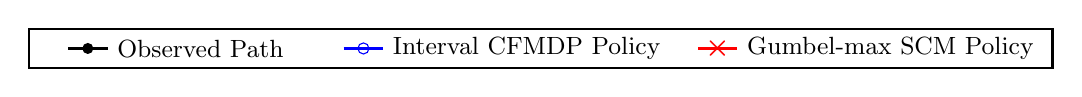
\begin{tikzpicture}[scale=1.0, every node/.style={scale=1.0}]
            \draw[thick, black] (-3, -0.25) rectangle (10, 0.25);
            %
            \draw[black, line width=1pt] (-2.5, 0.0) -- (-2,0.0);
            \fill[black] (-2.25,0.0) circle (2pt); %
            \node[right] at (-2,0.0) {\small Observed Path};
            
            %
            \draw[blue, line width=1pt] (1.0,0.0) -- (1.5,0.0);
            \node[draw=blue, circle, minimum size=4pt, inner sep=0pt] at (1.25,0.0) {}; %
            \node[right] at (1.5,0.0) {\small Interval CFMDP Policy};
            
            %
            \draw[red, line width=1pt] (5.5,0) -- (6,0);
            \node[red] at (5.75,0) {$\boldsymbol{\times}$}; %
            \node[right] at (6,0) {\small Gumbel-max SCM Policy};
        \end{tikzpicture}
    }\\
    %
    \subfigure[\footnotesize Lowest cumulative reward: Interval CFMDP ($312$), Gumbel-max SCM ($312$)]{%
        \resizebox{0.76\columnwidth}{!}{
             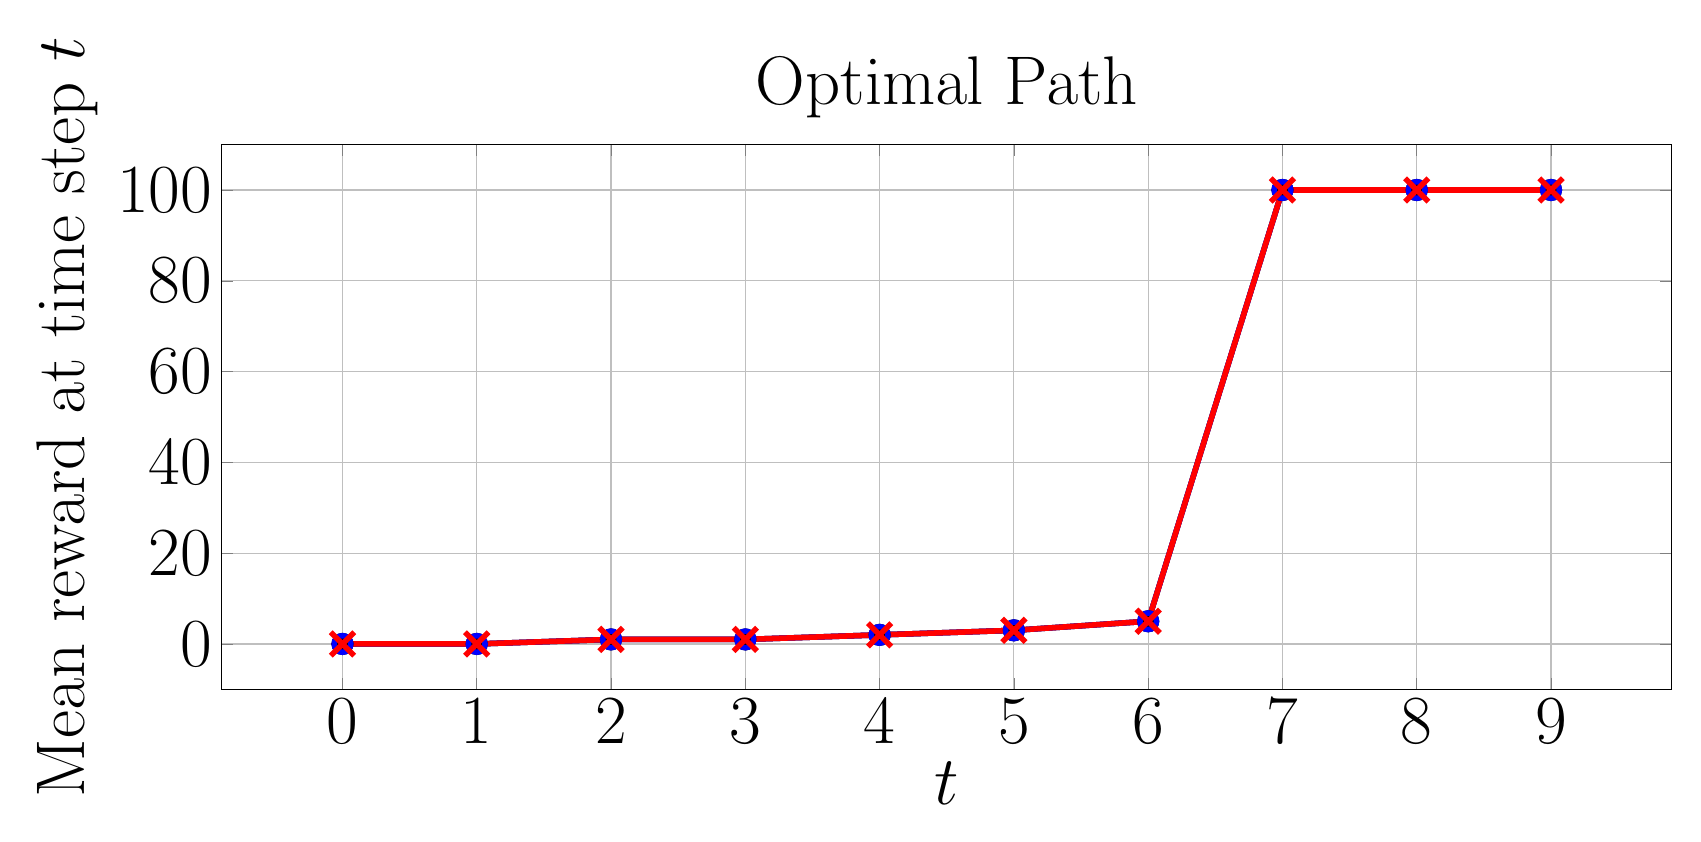
\begin{tikzpicture}
                \begin{axis}[
                    xlabel={$t$},
                    ylabel={Mean reward at time step $t$},
                    title={Optimal Path},
                    grid=both,
                    width=20cm, height=8.5cm,
                    every axis/.style={font=\Huge},
                    %
                ]
                \addplot[
                    color=black, %
                    mark=*, %
                    line width=2pt,
                    mark size=3pt,
                    error bars/.cd,
                    y dir=both, %
                    y explicit, %
                    error bar style={line width=1pt,solid},
                    error mark options={line width=1pt,mark size=4pt,rotate=90}
                ]
                coordinates {
                    (0, 0.0)  +- (0, 0.0)
                    (1, 0.0)  +- (0, 0.0) 
                    (2, 1.0)  +- (0, 0.0) 
                    (3, 1.0)  +- (0, 0.0)
                    (4, 2.0)  +- (0, 0.0)
                    (5, 3.0) +- (0, 0.0)
                    (6, 5.0) +- (0, 0.0)
                    (7, 100.0) +- (0, 0.0)
                    (8, 100.0) +- (0, 0.0)
                    (9, 100.0) +- (0, 0.0)
                };
                %
                \addplot[
                    color=blue, %
                    mark=o, %
                    line width=2pt,
                    mark size=3pt,
                    error bars/.cd,
                    y dir=both, %
                    y explicit, %
                    error bar style={line width=1pt,solid},
                    error mark options={line width=1pt,mark size=4pt,rotate=90}
                ]
                 coordinates {
                    (0, 0.0)  +- (0, 0.0)
                    (1, 0.0)  +- (0, 0.0) 
                    (2, 1.0)  +- (0, 0.0) 
                    (3, 1.0)  +- (0, 0.0)
                    (4, 2.0)  +- (0, 0.0)
                    (5, 3.0) +- (0, 0.0)
                    (6, 5.0) +- (0, 0.0)
                    (7, 100.0) +- (0, 0.0)
                    (8, 100.0) +- (0, 0.0)
                    (9, 100.0) +- (0, 0.0)
                };
                %
                \addplot[
                    color=red, %
                    mark=x, %
                    line width=2pt,
                    mark size=6pt,
                    error bars/.cd,
                    y dir=both, %
                    y explicit, %
                    error bar style={line width=1pt,solid},
                    error mark options={line width=1pt,mark size=4pt,rotate=90}
                ]
                coordinates {
                    (0, 0.0)  +- (0, 0.0)
                    (1, 0.0)  +- (0, 0.0) 
                    (2, 1.0)  +- (0, 0.0) 
                    (3, 1.0)  +- (0, 0.0)
                    (4, 2.0)  +- (0, 0.0)
                    (5, 3.0) +- (0, 0.0)
                    (6, 5.0) +- (0, 0.0)
                    (7, 100.0) +- (0, 0.0)
                    (8, 100.0) +- (0, 0.0)
                    (9, 100.0) +- (0, 0.0)
                };
                \end{axis}
            \end{tikzpicture}
         }
    }
    \hspace{1cm}
    \subfigure[\footnotesize Lowest cumulative reward: Interval CFMDP ($19$), Gumbel-max SCM ($-88$)]{%
         \resizebox{0.76\columnwidth}{!}{
            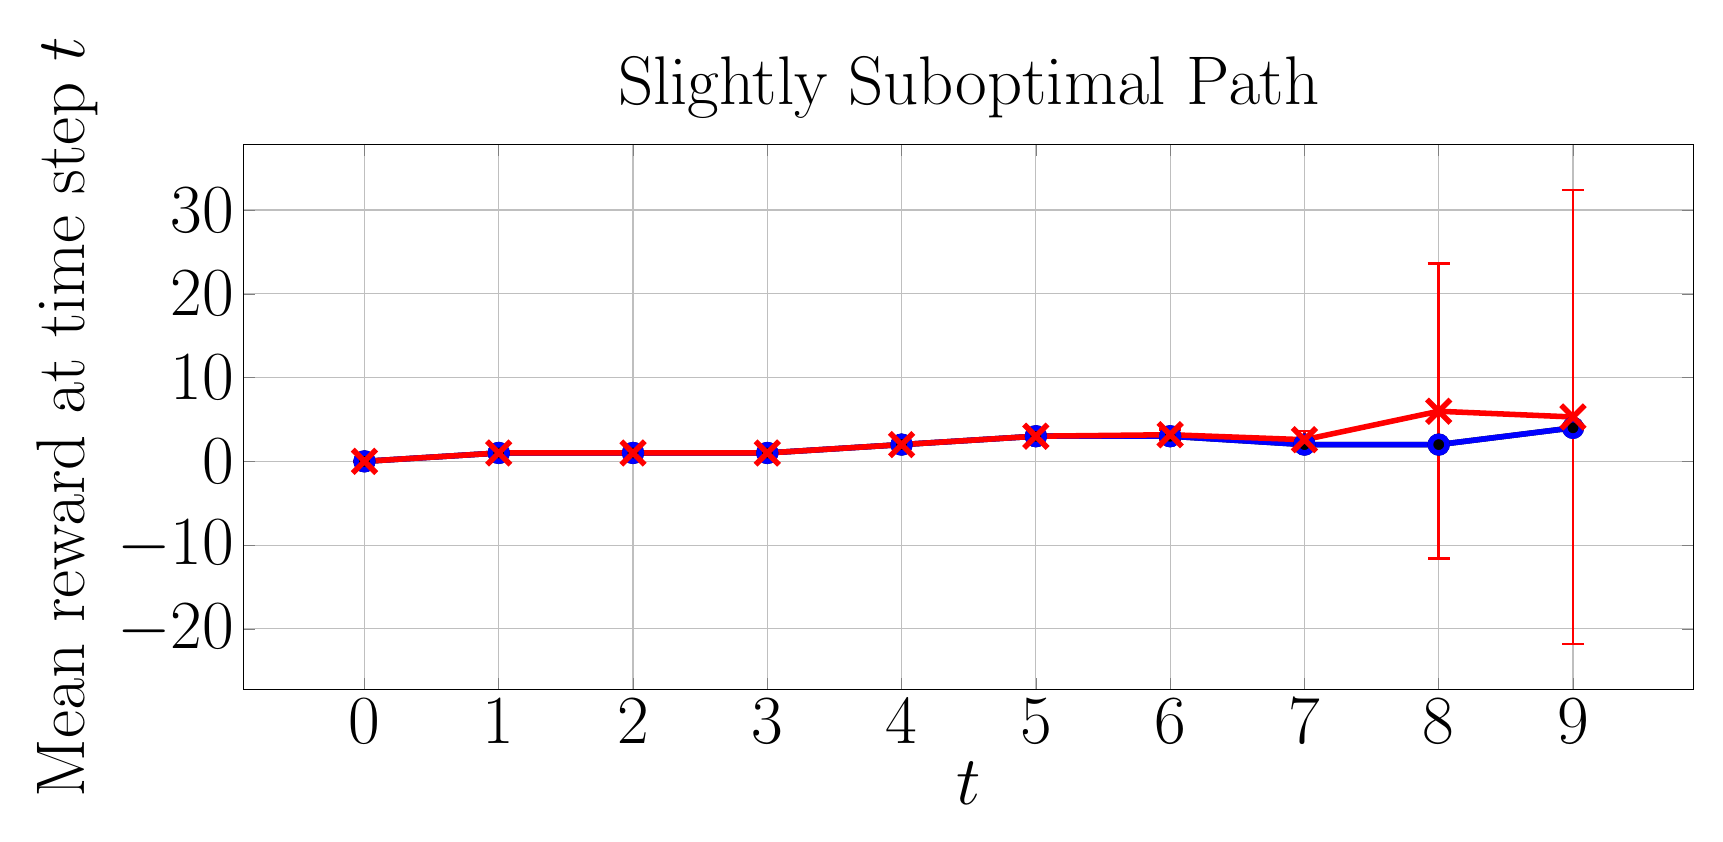
\begin{tikzpicture}
                \begin{axis}[
                    xlabel={$t$},
                    ylabel={Mean reward at time step $t$},
                    title={Slightly Suboptimal Path},
                    grid=both,
                    width=20cm, height=8.5cm,
                    every axis/.style={font=\Huge},
                    %
                ]
                \addplot[
                    color=black, %
                    mark=*, %
                    line width=2pt,
                    mark size=3pt,
                    error bars/.cd,
                    y dir=both, %
                    y explicit, %
                    error bar style={line width=1pt,solid},
                    error mark options={line width=1pt,mark size=4pt,rotate=90}
                ]
              coordinates {
                    (0, 0.0)  +- (0, 0.0)
                    (1, 1.0)  +- (0, 0.0) 
                    (2, 1.0)  +- (0, 0.0) 
                    (3, 1.0)  +- (0, 0.0)
                    (4, 2.0)  +- (0, 0.0)
                    (5, 3.0) +- (0, 0.0)
                    (6, 3.0) +- (0, 0.0)
                    (7, 2.0) +- (0, 0.0)
                    (8, 2.0) +- (0, 0.0)
                    (9, 4.0) +- (0, 0.0)
                };
                %
                \addplot[
                    color=blue, %
                    mark=o, %
                    line width=2pt,
                    mark size=3pt,
                    error bars/.cd,
                    y dir=both, %
                    y explicit, %
                    error bar style={line width=1pt,solid},
                    error mark options={line width=1pt,mark size=4pt,rotate=90}
                ]
              coordinates {
                    (0, 0.0)  +- (0, 0.0)
                    (1, 1.0)  +- (0, 0.0) 
                    (2, 1.0)  +- (0, 0.0) 
                    (3, 1.0)  +- (0, 0.0)
                    (4, 2.0)  +- (0, 0.0)
                    (5, 3.0) +- (0, 0.0)
                    (6, 3.0) +- (0, 0.0)
                    (7, 2.0) +- (0, 0.0)
                    (8, 2.0) +- (0, 0.0)
                    (9, 4.0) +- (0, 0.0)
                };
                %
                \addplot[
                    color=red, %
                    mark=x, %
                    line width=2pt,
                    mark size=6pt,
                    error bars/.cd,
                    y dir=both, %
                    y explicit, %
                    error bar style={line width=1pt,solid},
                    error mark options={line width=1pt,mark size=4pt,rotate=90}
                ]
                coordinates {
                    (0, 0.0)  +- (0, 0.0)
                    (1, 1.0)  +- (0, 0.0) 
                    (2, 1.0)  +- (0, 0.0) 
                    (3, 1.0)  +- (0, 0.0)
                    (4, 2.0)  += (0, 0.0)
                    (5, 3.0)  += (0, 0.0)
                    (6, 3.17847) += (0, 0.62606746) -= (0, 0.62606746)
                    (7, 2.5832885) += (0, 1.04598233) -= (0, 1.04598233)
                    (8, 5.978909) += (0, 17.60137623) -= (0, 17.60137623)
                    (9, 5.297059) += (0, 27.09227512) -= (0, 27.09227512)
                };
                \end{axis}
            \end{tikzpicture}
         }
    }\\[-1.5pt]
    \subfigure[\footnotesize Lowest cumulative reward: Interval CFMDP ($14$), Gumbel-max SCM ($-598$)]{%
         \resizebox{0.76\columnwidth}{!}{
             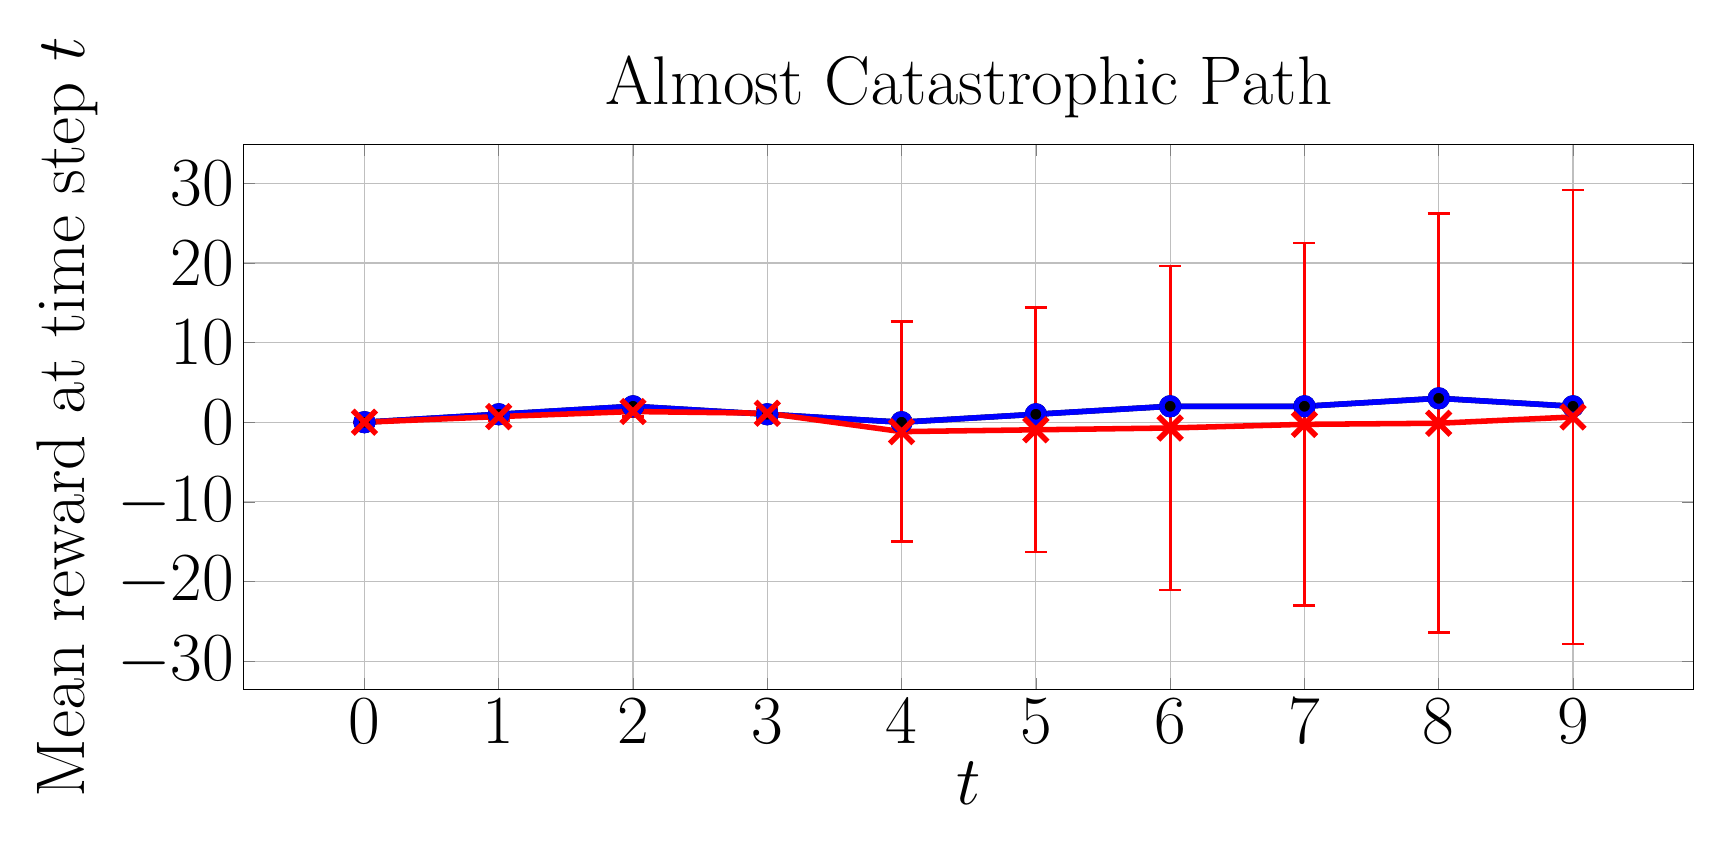
\begin{tikzpicture}
                \begin{axis}[
                    xlabel={$t$},
                    ylabel={Mean reward at time step $t$},
                    title={Almost Catastrophic Path},
                    grid=both,
                    width=20cm, height=8.5cm,
                    every axis/.style={font=\Huge},
                    %
                ]
                \addplot[
                    color=black, %
                    mark=*, %
                    line width=2pt,
                    mark size=3pt,
                    error bars/.cd,
                    y dir=both, %
                    y explicit, %
                    error bar style={line width=1pt,solid},
                    error mark options={line width=1pt,mark size=4pt,rotate=90}
                ]
                coordinates {
                    (0, 0.0)  +- (0, 0.0)
                    (1, 1.0)  +- (0, 0.0) 
                    (2, 2.0)  +- (0, 0.0) 
                    (3, 1.0)  +- (0, 0.0)
                    (4, 0.0)  +- (0, 0.0)
                    (5, 1.0) +- (0, 0.0)
                    (6, 2.0) +- (0, 0.0)
                    (7, 2.0) +- (0, 0.0)
                    (8, 3.0) +- (0, 0.0)
                    (9, 2.0) +- (0, 0.0)
                };
                %
                \addplot[
                    color=blue, %
                    mark=o, %
                    line width=2pt,
                    mark size=3pt,
                    error bars/.cd,
                    y dir=both, %
                    y explicit, %
                    error bar style={line width=1pt,solid},
                    error mark options={line width=1pt,mark size=4pt,rotate=90}
                ]
                coordinates {
                    (0, 0.0)  +- (0, 0.0)
                    (1, 1.0)  +- (0, 0.0) 
                    (2, 2.0)  +- (0, 0.0) 
                    (3, 1.0)  +- (0, 0.0)
                    (4, 0.0)  +- (0, 0.0)
                    (5, 1.0) +- (0, 0.0)
                    (6, 2.0) +- (0, 0.0)
                    (7, 2.0) +- (0, 0.0)
                    (8, 3.0) +- (0, 0.0)
                    (9, 2.0) +- (0, 0.0)
                };
                %
                \addplot[
                    color=red, %
                    mark=x, %
                    line width=2pt,
                    mark size=6pt,
                    error bars/.cd,
                    y dir=both, %
                    y explicit, %
                    error bar style={line width=1pt,solid},
                    error mark options={line width=1pt,mark size=4pt,rotate=90}
                ]
                coordinates {
                    (0, 0.0)  +- (0, 0.0)
                    (1, 0.7065655)  +- (0, 0.4553358) 
                    (2, 1.341673)  +- (0, 0.67091621) 
                    (3, 1.122926)  +- (0, 0.61281824)
                    (4, -1.1821935)  +- (0, 13.82444042)
                    (5, -0.952399)  +- (0, 15.35195457)
                    (6, -0.72672) +- (0, 20.33508414)
                    (7, -0.268983) +- (0, 22.77861454)
                    (8, -0.1310835) +- (0, 26.31013314)
                    (9, 0.65806) +- (0, 28.50670214)
                };
                %
            %
            %
            %
            %
            %
            %
            %
            %
            %
            %
            %
            %
            %
            %
            %
            %
            %
            %
                \end{axis}
            \end{tikzpicture}
         }
    }
    \hspace{1cm}
    \subfigure[\footnotesize Lowest cumulative reward: Interval CFMDP ($-698$), Gumbel-max SCM ($-698$)]{%
         \resizebox{0.76\columnwidth}{!}{
            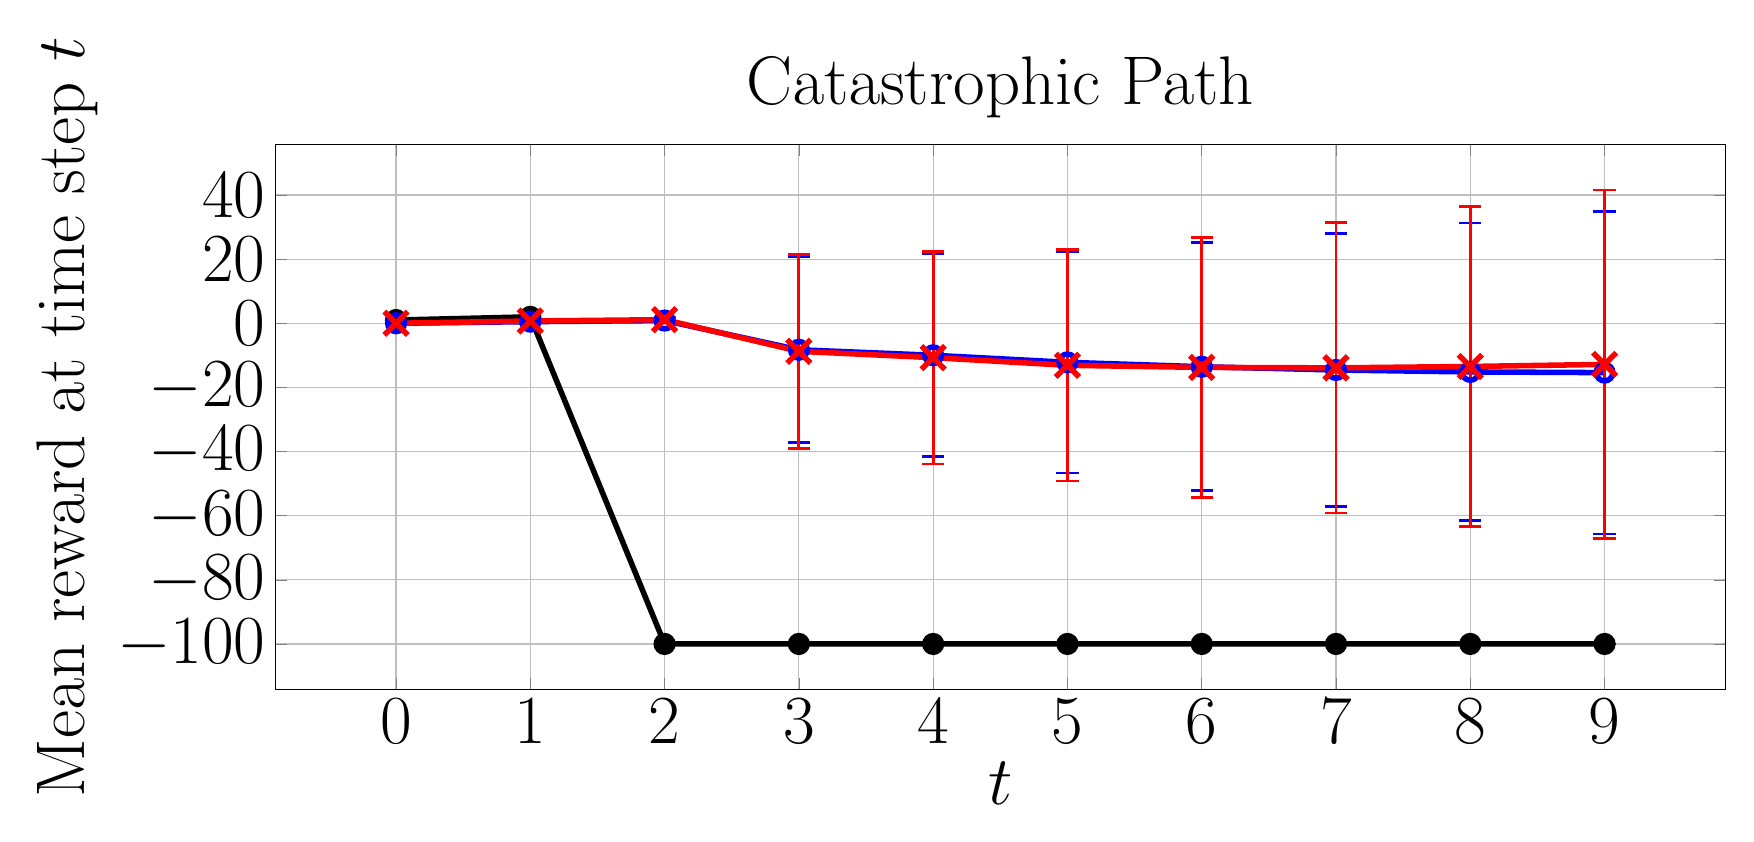
\begin{tikzpicture}
                \begin{axis}[
                    xlabel={$t$},
                    ylabel={Mean reward at time step $t$},
                    title={Catastrophic Path},
                    grid=both,
                    width=20cm, height=8.5cm,
                    every axis/.style={font=\Huge},
                    %
                ]
                \addplot[
                    color=black, %
                    mark=*, %
                    line width=2pt,
                    mark size=3pt,
                    error bars/.cd,
                    y dir=both, %
                    y explicit, %
                    error bar style={line width=1pt,solid},
                    error mark options={line width=1pt,mark size=4pt,rotate=90}
                ]
                coordinates {
                    (0, 1.0)  +- (0, 0.0)
                    (1, 2.0)  +- (0, 0.0) 
                    (2, -100.0)  +- (0, 0.0) 
                    (3, -100.0)  +- (0, 0.0)
                    (4, -100.0)  +- (0, 0.0)
                    (5, -100.0) +- (0, 0.0)
                    (6, -100.0) +- (0, 0.0)
                    (7, -100.0) +- (0, 0.0)
                    (8, -100.0) +- (0, 0.0)
                    (9, -100.0) +- (0, 0.0)
                };
                %
                \addplot[
                    color=blue, %
                    mark=o, %
                    line width=2pt,
                    mark size=3pt,
                    error bars/.cd,
                    y dir=both, %
                    y explicit, %
                    error bar style={line width=1pt,solid},
                    error mark options={line width=1pt,mark size=4pt,rotate=90}
                ]
                coordinates {
                    (0, 0.0)  +- (0, 0.0)
                    (1, 0.504814)  +- (0, 0.49997682) 
                    (2, 0.8439835)  +- (0, 0.76831917) 
                    (3, -8.2709165)  +- (0, 28.93656754)
                    (4, -9.981082)  +- (0, 31.66825363)
                    (5, -12.1776325) +- (0, 34.53463233)
                    (6, -13.556076) +- (0, 38.62845372)
                    (7, -14.574418) +- (0, 42.49603359)
                    (8, -15.1757075) +- (0, 46.41913968)
                    (9, -15.3900395) +- (0, 50.33563368)
                };
                %
                \addplot[
                    color=red, %
                    mark=x, %
                    line width=2pt,
                    mark size=6pt,
                    error bars/.cd,
                    y dir=both, %
                    y explicit, %
                    error bar style={line width=1pt,solid},
                    error mark options={line width=1pt,mark size=4pt,rotate=90}
                ]
                coordinates {
                    (0, 0.0)  +- (0, 0.0)
                    (1, 0.701873)  +- (0, 0.45743556) 
                    (2, 1.1227805)  +- (0, 0.73433129) 
                    (3, -8.7503255)  +- (0, 30.30257976)
                    (4, -10.722092)  +- (0, 33.17618589)
                    (5, -13.10721)  +- (0, 36.0648089)
                    (6, -13.7631645) +- (0, 40.56553451)
                    (7, -13.909043) +- (0, 45.23829402)
                    (8, -13.472517) +- (0, 49.96270296)
                    (9, -12.8278835) +- (0, 54.38618735)
                };
                %
            %
            %
            %
            %
            %
            %
            %
            %
            %
            %
            %
            %
            %
            %
            %
            %
            %
            %
                \end{axis}
            \end{tikzpicture}
         }
    }
    \caption{Average instant reward of CF paths induced by policies on GridWorld $p=0.4$.}
    \label{fig: reward p=0.4}
\end{figure*}

\subsection{Experimental Setup}
To compare policy performance, we measure the average rewards of counterfactual paths induced by our policy and the Gumbel-max policy by uniformly sampling $200$ counterfactual MDPs from the ICFMDP and generating $10,000$ counterfactual paths over each sampled CFMDP. \jl{Since the interval CFMDP depends on the observed path, we select $4$  paths of varying optimality to evaluate how the observed path impacts the performance of both policies: an optimal path, a slightly suboptimal path that could reach the optimal reward with a few changes, a catastrophic path that enters a catastrophic, terminal state with low reward, and an almost catastrophic path that was close to entering a catastrophic state.} When measuring the average probability bound widths and execution time needed to generate the ICFMDPs, we averaged over $20$ randomly generated observed paths
\footnote{Further training details are provided in Appendix \ref{app: training details}, and the code is provided at \href{https://github.com/ddv-lab/robust-cf-inference-in-MDPs}{https://github.com/ddv-lab/robust-cf-inference-in-MDPs}
%
%
.}.

\subsection{GridWorld}
\jl{The GridWorld MDP is a $4 \times 4$ grid where an agent must navigate from the top-left corner to the goal state in the bottom-right corner, avoiding a dangerous terminal state in the centre. At each time step, the agent can move up, down, left, or right, but there is a small probability (controlled by hyper-parameter $p$) of moving in an unintended direction. As the agent nears the goal, the reward for each state increases, culminating in a reward of $+100$ for reaching the goal. Entering the dangerous state results in a penalty of $-100$. We use two versions of GridWorld: a less stochastic version with $p=0.9$ (i.e., $90$\% chance of moving in the chosen direction) and a more stochastic version with $p=0.4$.}

\paragraph{GridWorld ($p=0.9$)}
When $p=0.9$, the counterfactual probability bounds are typically narrow (see Table \ref{tab:nonzero_probs} for average measurements). Consequently, as shown in Figure \ref{fig: reward p=0.9}, both policies are nearly identical and perform similarly well across the optimal, slightly suboptimal, and catastrophic paths.
%
However, for the almost catastrophic path, the interval CFMDP path is more conservative and follows the observed path more closely (as this is where the probability bounds are narrowest), which typically requires one additional step to reach the goal state than the Gumbel-max SCM policy.
%

\paragraph{GridWorld ($p=0.4$)}
\jl{When $p=0.4$, the GridWorld environment becomes more uncertain, increasing the risk of entering the dangerous state even if correct actions are chosen. Thus, as shown in Figure \ref{fig: reward p=0.4}, the interval CFMDP policy adopts a more conservative approach, avoiding deviation from the observed policy if it cannot guarantee higher counterfactual rewards (see the slightly suboptimal and almost catastrophic paths), whereas the Gumbel-max SCM is inconsistent: it can yield higher rewards, but also much lower rewards, reflected in the wide error bars.} For the catastrophic path, both policies must deviate from the observed path to achieve a higher reward and, in this case, perform similarly.
%
%
%
%
\subsection{Sepsis}
The Sepsis MDP \citep{oberst2019counterfactual} simulates trajectories of Sepsis patients. Each state consists of four vital signs (heart rate, blood pressure, oxygen concentration, and glucose levels), categorised as low, normal, or high.
and three treatments that can be toggled on/off at each time step (8 actions in total). Unlike \citet{oberst2019counterfactual}, we scale rewards based on the number of out-of-range vital signs, between $-1000$ (patient dies) and $1000$ (patient discharged). \jl{Like the GridWorld $p=0.4$ experiment, the Sepsis MDP is highly uncertain, as many states are equally likely to lead to optimal and poor outcomes. Thus, as shown in Figure \ref{fig: reward sepsis}, both policies follow the observed optimal and almost catastrophic paths to guarantee rewards are no worse than the observation.} However, improving the catastrophic path requires deviating from the observation. Here, the Gumbel-max SCM policy, on average, performs better than the interval CFMDP policy. But, since both policies have lower bounds clipped at $-1000$, neither policy reliably improves over the observation. In contrast, for the slightly suboptimal path, the interval CFMDP policy performs significantly better, shown by its higher lower bounds. 
Moreover, in these two cases, the worst-case counterfactual path generated by the interval CFMDP policy is better than that of the Gumbel-max SCM policy,
indicating its greater robustness.
%
\begin{figure*}
    \centering
     \resizebox{0.6\textwidth}{!}{
        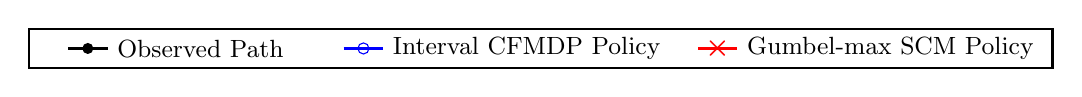
\begin{tikzpicture}[scale=1.0, every node/.style={scale=1.0}]
            \draw[thick, black] (-3, -0.25) rectangle (10, 0.25);
            %
            \draw[black, line width=1pt] (-2.5, 0.0) -- (-2,0.0);
            \fill[black] (-2.25,0.0) circle (2pt); %
            \node[right] at (-2,0.0) {\small Observed Path};
            
            %
            \draw[blue, line width=1pt] (1.0,0.0) -- (1.5,0.0);
            \node[draw=blue, circle, minimum size=4pt, inner sep=0pt] at (1.25,0.0) {}; %
            \node[right] at (1.5,0.0) {\small Interval CFMDP Policy};
            
            %
            \draw[red, line width=1pt] (5.5,0) -- (6,0);
            \node[red] at (5.75,0) {$\boldsymbol{\times}$}; %
            \node[right] at (6,0) {\small Gumbel-max SCM Policy};
        \end{tikzpicture}
    }\\
    \subfigure[\footnotesize Lowest cumulative reward: Interval CFMDP ($8000$), Gumbel-max SCM ($8000$)]{%
         \resizebox{0.76\columnwidth}{!}{
             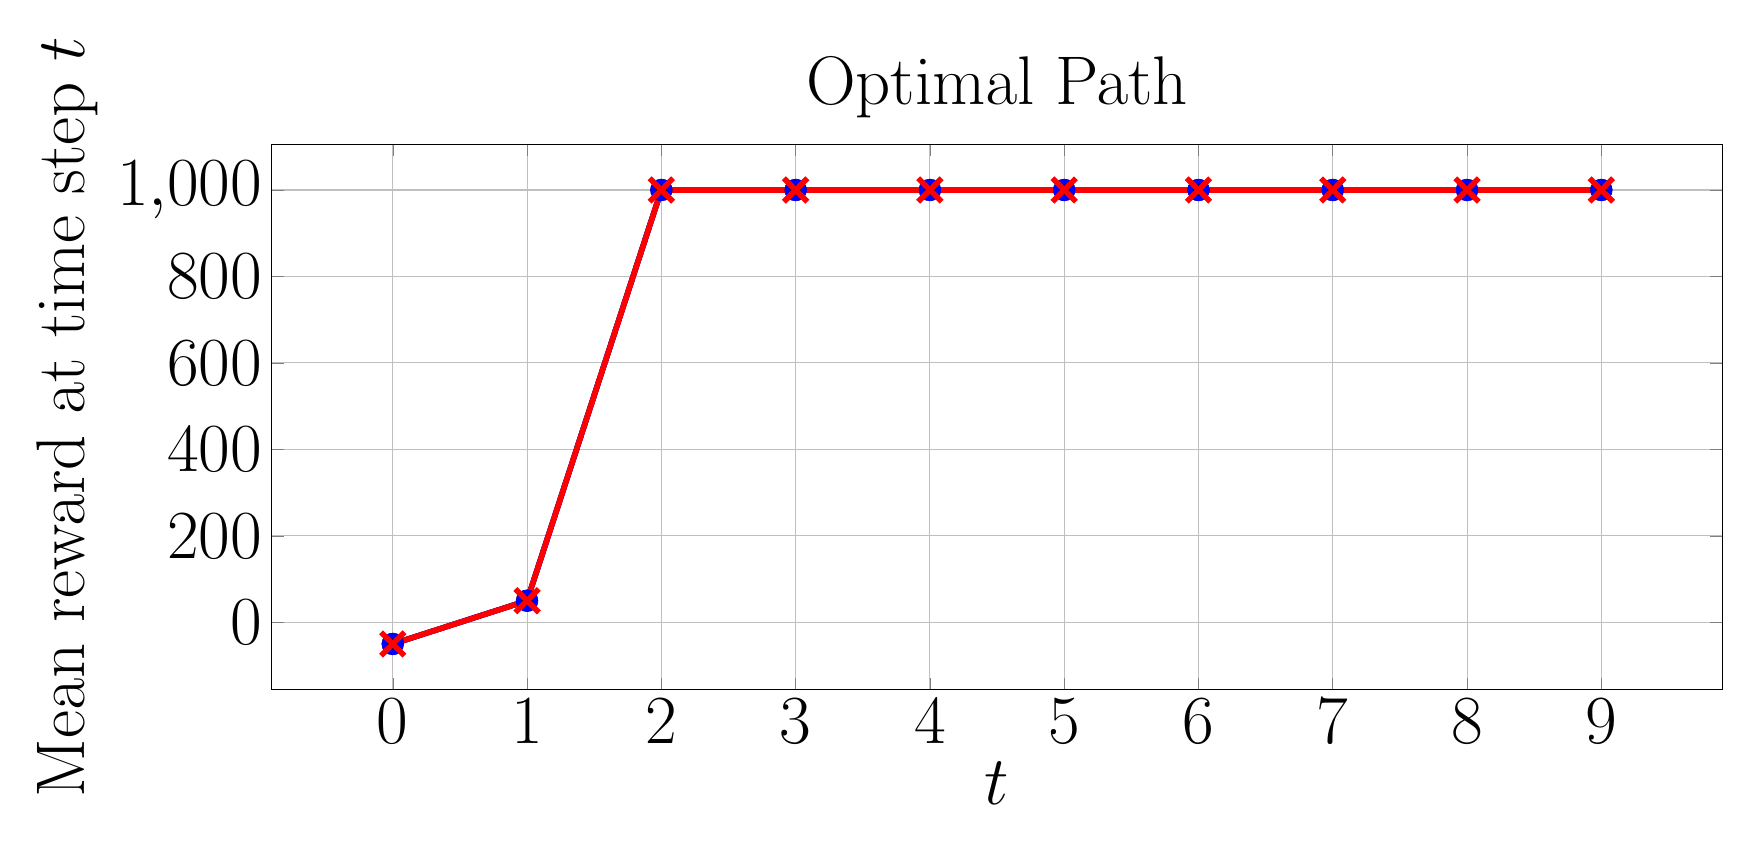
\begin{tikzpicture}
                \begin{axis}[
                    xlabel={$t$},
                    ylabel={Mean reward at time step $t$},
                    title={Optimal Path},
                    grid=both,
                    width=20cm, height=8.5cm,
                    every axis/.style={font=\Huge},
                    %
                ]
                \addplot[
                    color=black, %
                    mark=*, %
                    line width=2pt,
                    mark size=3pt,
                ]
                coordinates {
                    (0, -50.0)
                    (1, 50.0)
                    (2, 1000.0)
                    (3, 1000.0)
                    (4, 1000.0)
                    (5, 1000.0)
                    (6, 1000.0)
                    (7, 1000.0)
                    (8, 1000.0)
                    (9, 1000.0)
                };
                %
                \addplot[
                    color=blue, %
                    mark=o, %
                    line width=2pt,
                    mark size=3pt,
                    error bars/.cd,
                    y dir=both, %
                    y explicit, %
                    error bar style={line width=1pt,solid},
                    error mark options={line width=1pt,mark size=4pt,rotate=90}
                ]
                coordinates {
                    (0, -50.0)  +- (0, 0.0)
                    (1, 50.0)  +- (0, 0.0) 
                    (2, 1000.0)  +- (0, 0.0) 
                    (3, 1000.0)  +- (0, 0.0)
                    (4, 1000.0)  +- (0, 0.0)
                    (5, 1000.0) +- (0, 0.0)
                    (6, 1000.0) +- (0, 0.0)
                    (7, 1000.0) +- (0, 0.0)
                    (8, 1000.0) +- (0, 0.0)
                    (9, 1000.0) +- (0, 0.0)
                };
                %
                \addplot[
                    color=red, %
                    mark=x, %
                    line width=2pt,
                    mark size=6pt,
                    error bars/.cd,
                    y dir=both, %
                    y explicit, %
                    error bar style={line width=1pt,solid},
                    error mark options={line width=1pt,mark size=4pt,rotate=90}
                ]
                coordinates {
                    (0, -50.0)  +- (0, 0.0)
                    (1, 50.0)  +- (0, 0.0) 
                    (2, 1000.0)  +- (0, 0.0) 
                    (3, 1000.0)  +- (0, 0.0)
                    (4, 1000.0)  +- (0, 0.0)
                    (5, 1000.0) +- (0, 0.0)
                    (6, 1000.0) +- (0, 0.0)
                    (7, 1000.0) +- (0, 0.0)
                    (8, 1000.0) +- (0, 0.0)
                    (9, 1000.0) +- (0, 0.0)
                };
                %
                \end{axis}
            \end{tikzpicture}
         }
    }
    \hspace{1cm}
    \subfigure[\footnotesize Lowest cumulative reward: Interval CFMDP ($-5980$), Gumbel-max SCM ($-8000$)]{%
         \resizebox{0.76\columnwidth}{!}{
            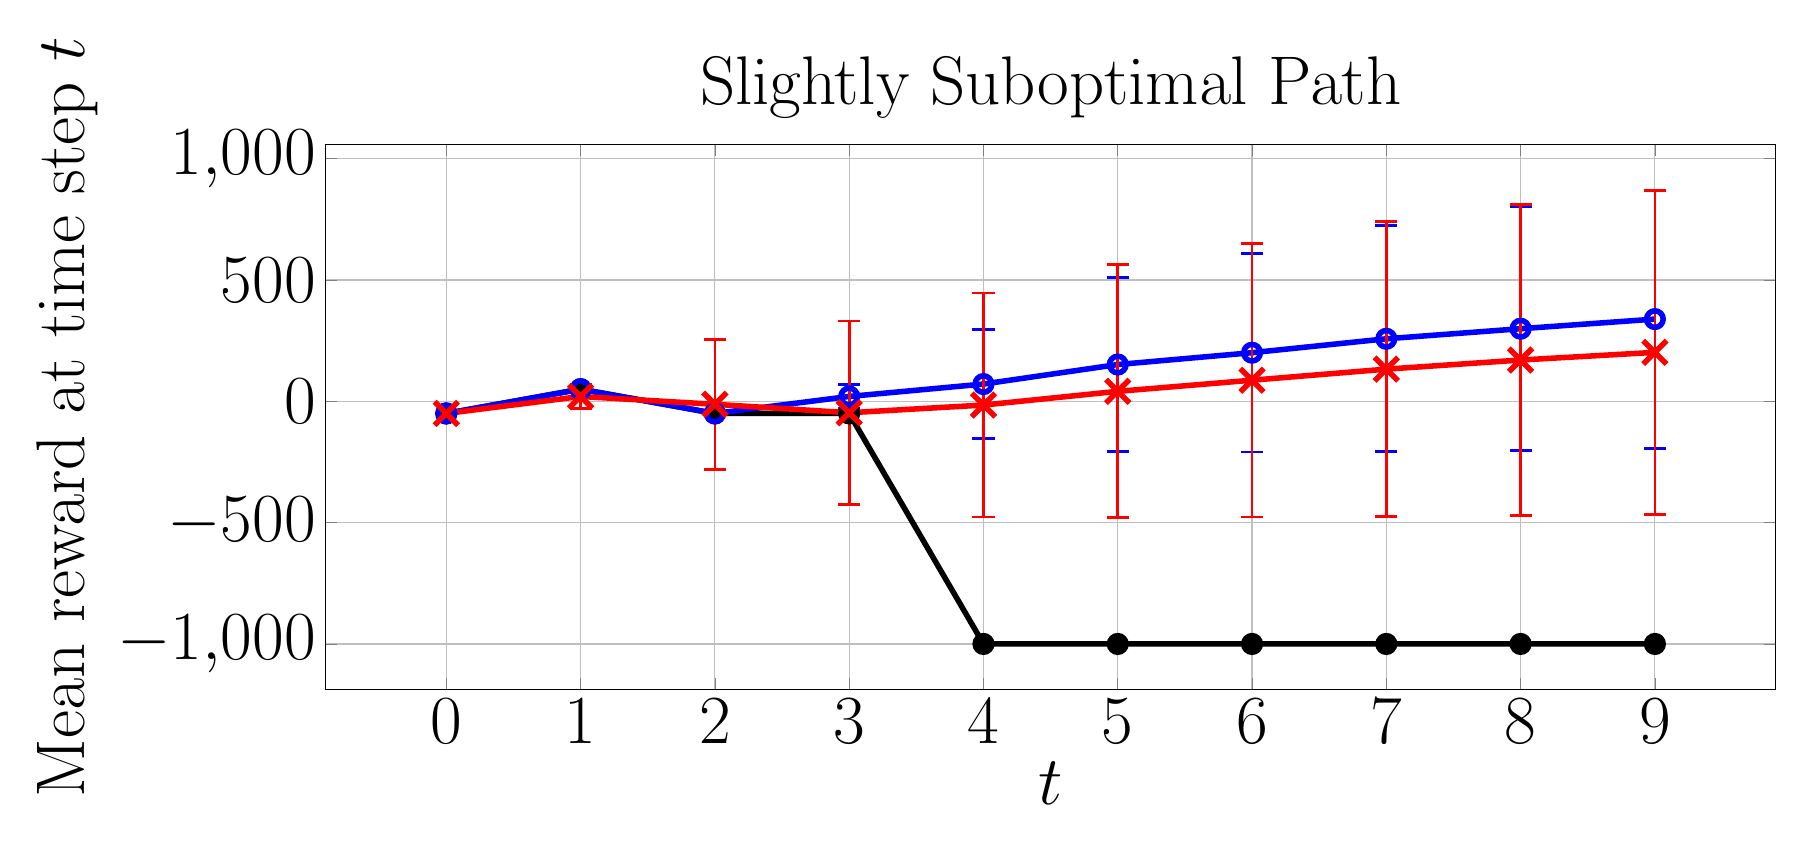
\begin{tikzpicture}
                \begin{axis}[
                    xlabel={$t$},
                    ylabel={Mean reward at time step $t$},
                    title={Slightly Suboptimal Path},
                    grid=both,
                    width=20cm, height=8.5cm,
                    every axis/.style={font=\Huge},
                    %
                ]
               \addplot[
                    color=black, %
                    mark=*, %
                    line width=2pt,
                    mark size=3pt,
                ]
                coordinates {
                    (0, -50.0)
                    (1, 50.0)
                    (2, -50.0)
                    (3, -50.0)
                    (4, -1000.0)
                    (5, -1000.0)
                    (6, -1000.0)
                    (7, -1000.0)
                    (8, -1000.0)
                    (9, -1000.0)
                };
                %
                \addplot[
                    color=blue, %
                    mark=o, %
                    line width=2pt,
                    mark size=3pt,
                    error bars/.cd,
                    y dir=both, %
                    y explicit, %
                    error bar style={line width=1pt,solid},
                    error mark options={line width=1pt,mark size=4pt,rotate=90}
                ]
                coordinates {
                    (0, -50.0)  +- (0, 0.0)
                    (1, 50.0)  +- (0, 0.0) 
                    (2, -50.0)  +- (0, 0.0) 
                    (3, 20.0631)  +- (0, 49.97539413)
                    (4, 71.206585)  +- (0, 226.02033693)
                    (5, 151.60797) +- (0, 359.23292559)
                    (6, 200.40593) +- (0, 408.86185176)
                    (7, 257.77948) +- (0, 466.10372804)
                    (8, 299.237465) +- (0, 501.82579506)
                    (9, 338.9129) +- (0, 532.06124996)
                };
                %
                \addplot[
                    color=red, %
                    mark=x, %
                    line width=2pt,
                    mark size=6pt,
                    error bars/.cd,
                    y dir=both, %
                    y explicit, %
                    error bar style={line width=1pt,solid},
                    error mark options={line width=1pt,mark size=4pt,rotate=90}
                ]
                coordinates {
                    (0, -50.0)  +- (0, 0.0)
                    (1, 20.00736)  +- (0, 49.99786741) 
                    (2, -12.282865)  +- (0, 267.598755) 
                    (3, -47.125995)  +- (0, 378.41755832)
                    (4, -15.381965)  +- (0, 461.77616558)
                    (5, 41.15459) +- (0, 521.53189262)
                    (6, 87.01595) +- (0, 564.22243126 )
                    (7, 132.62376) +- (0, 607.31338037)
                    (8, 170.168145) +- (0, 641.48013693)
                    (9, 201.813135) +- (0, 667.29441777)
                };
                %
                %
                %
                %
                %
                %
                %
                %
                %
                %
                %
                %
                %
                %
                %
                %
                %
                %
                %
                \end{axis}
            \end{tikzpicture}
         }
    }\\[-1.5pt]
    \subfigure[\footnotesize Lowest cumulative reward: Interval CFMDP ($100$), Gumbel-max SCM ($100$)]{%
         \resizebox{0.76\columnwidth}{!}{
             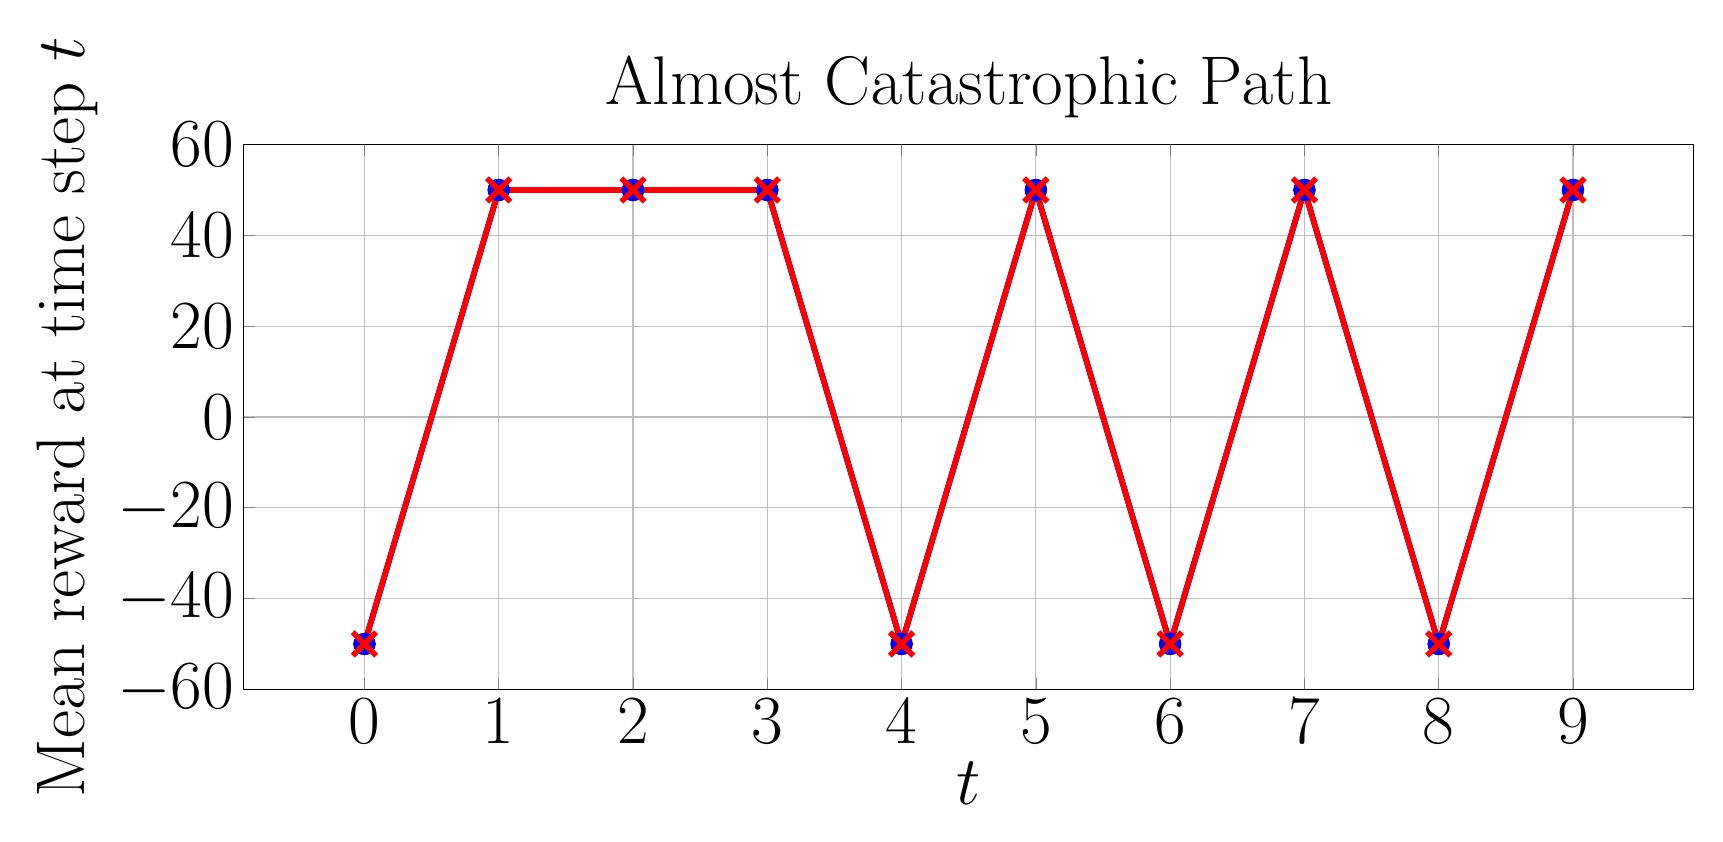
\begin{tikzpicture}
                \begin{axis}[
                    xlabel={$t$},
                    ylabel={Mean reward at time step $t$},
                    title={Almost Catastrophic Path},
                    grid=both,
                    every axis/.style={font=\Huge},
                    width=20cm, height=8.5cm,
                    %
                ]
               \addplot[
                    color=black, %
                    mark=*, %
                    line width=2pt,
                    mark size=3pt,
                ]
                coordinates {
                    (0, -50.0)
                    (1, 50.0)
                    (2, 50.0)
                    (3, 50.0)
                    (4, -50.0)
                    (5, 50.0)
                    (6, -50.0)
                    (7, 50.0)
                    (8, -50.0)
                    (9, 50.0)
                };
                %
                %
                \addplot[
                    color=blue, %
                    mark=o, %
                    line width=2pt,
                    mark size=3pt,
                    error bars/.cd,
                    y dir=both, %
                    y explicit, %
                    error bar style={line width=1pt,solid},
                    error mark options={line width=1pt,mark size=4pt,rotate=90}
                ]
                coordinates {
                    (0, -50.0)  +- (0, 0.0)
                    (1, 50.0)  +- (0, 0.0) 
                    (2, 50.0)  +- (0, 0.0) 
                    (3, 50.0)  +- (0, 0.0)
                    (4, -50.0)  +- (0, 0.0)
                    (5, 50.0) +- (0, 0.0)
                    (6, -50.0) +- (0, 0.0)
                    (7, 50.0) +- (0, 0.0)
                    (8, -50.0) +- (0, 0.0)
                    (9, 50.0) +- (0, 0.0)
                };
                %
                \addplot[
                    color=red, %
                    mark=x, %
                    line width=2pt,
                    mark size=6pt,
                    error bars/.cd,
                    y dir=both, %
                    y explicit, %
                    error bar style={line width=1pt,solid},
                    error mark options={line width=1pt,mark size=4pt,rotate=90}
                ]
                coordinates {
                    (0, -50.0)  +- (0, 0.0)
                    (1, 50.0)  +- (0, 0.0) 
                    (2, 50.0)  +- (0, 0.0) 
                    (3, 50.0)  +- (0, 0.0)
                    (4, -50.0)  +- (0, 0.0)
                    (5, 50.0) +- (0, 0.0)
                    (6, -50.0) +- (0, 0.0)
                    (7, 50.0) +- (0, 0.0)
                    (8, -50.0) +- (0, 0.0)
                    (9, 50.0) +- (0, 0.0)
                };
                %
                %
                %
                %
                %
                %
                %
                %
                %
                %
                %
                %
                %
                %
                %
                %
                %
                %
                %
                \end{axis}
            \end{tikzpicture}
         }
    }
    \hspace{1cm}
    \subfigure[\footnotesize Lowest cumulative reward: Interval CFMDP ($-7150$), Gumbel-max SCM ($-9050$)]{%
         \resizebox{0.76\columnwidth}{!}{
            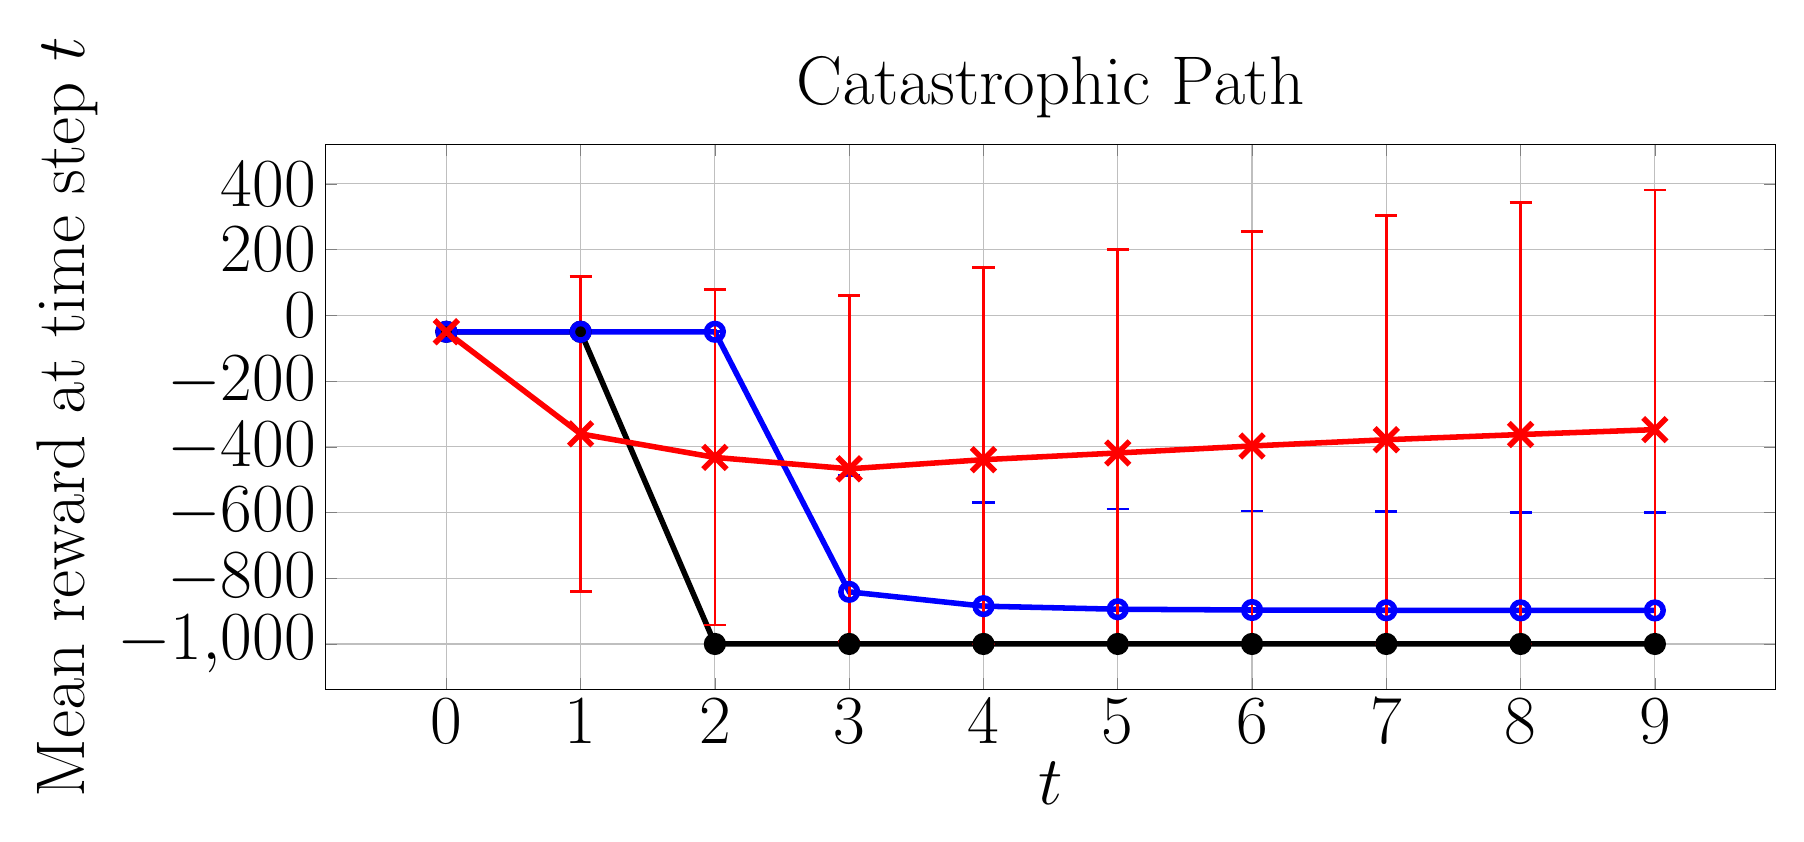
\begin{tikzpicture}
                \begin{axis}[
                    xlabel={$t$},
                    ylabel={Mean reward at time step $t$},
                    title={Catastrophic Path},
                    grid=both,
                    width=20cm, height=8.5cm,
                    every axis/.style={font=\Huge},
                    %
                ]
               \addplot[
                    color=black, %
                    mark=*, %
                    line width=2pt,
                    mark size=3pt,
                ]
                coordinates {
                    (0, -50.0)
                    (1, -50.0)
                    (2, -1000.0)
                    (3, -1000.0)
                    (4, -1000.0)
                    (5, -1000.0)
                    (6, -1000.0)
                    (7, -1000.0)
                    (8, -1000.0)
                    (9, -1000.0)
                };
                %
                %
                \addplot[
                    color=blue, %
                    mark=o, %
                    line width=2pt,
                    mark size=3pt,
                    error bars/.cd,
                    y dir=both, %
                    y explicit, %
                    error bar style={line width=1pt,solid},
                    error mark options={line width=1pt,mark size=4pt,rotate=90}
                ]
                coordinates {
                    (0, -50.0)  +- (0, 0.0)
                    (1, -50.0)  +- (0, 0.0) 
                    (2, -50.0)  +- (0, 0.0) 
                    (3, -841.440725)  += (0, 354.24605512) -= (0, 158.559275)
                    (4, -884.98225)  += (0, 315.37519669) -= (0, 115.01775)
                    (5, -894.330425) += (0, 304.88572805) -= (0, 105.669575)
                    (6, -896.696175) += (0, 301.19954514) -= (0, 103.303825)
                    (7, -897.4635) += (0, 299.61791279) -= (0, 102.5365)
                    (8, -897.77595) += (0, 298.80392585) -= (0, 102.22405)
                    (9, -897.942975) += (0, 298.32920557) -= (0, 102.057025)
                };
                %
                \addplot[
                    color=red, %
                    mark=x, %
                    line width=2pt,
                    mark size=6pt,
                    error bars/.cd,
                    y dir=both, %
                    y explicit, %
                    error bar style={line width=1pt,solid},
                    error mark options={line width=1pt,mark size=4pt,rotate=90}
                ]
            coordinates {
                    (0, -50.0)  +- (0, 0.0)
                    (1, -360.675265)  +- (0, 479.39812699) 
                    (2, -432.27629)  +- (0, 510.38620897) 
                    (3, -467.029545)  += (0, 526.36009628) -= (0, 526.36009628)
                    (4, -439.17429)  += (0, 583.96638919) -= (0, 560.82571)
                    (5, -418.82704) += (0, 618.43027478) -= (0, 581.17296)
                    (6, -397.464895) += (0, 652.67322574) -= (0, 602.535105)
                    (7, -378.49052) += (0, 682.85407033) -= (0, 621.50948)
                    (8, -362.654195) += (0, 707.01412023) -= (0, 637.345805)
                    (9, -347.737935) += (0, 729.29076479) -= (0, 652.262065)
                };
                %
                %
                %
                %
                %
                %
                %
                %
                %
                %
                %
                %
                %
                %
                %
                %
                %
                %
                %
                \end{axis}
            \end{tikzpicture}
         }
    }
    \caption{Average instant reward of CF paths induced by policies on Sepsis.}
    \label{fig: reward sepsis}
\end{figure*}

%
%
%
\subsection{Interval CFMDP Bounds}
%
%
Table \ref{tab:nonzero_probs} presents the mean counterfactual probability bound widths (excluding transitions where the upper bound is $0$) for each MDP, averaged over 20 observed paths. We compare the bounds under counterfactual stability (CS) and monotonicity (M) assumptions, CS alone, and no assumptions. This shows that the assumptions marginally reduce the bound widths, indicating the assumptions tighten the bounds without excluding too many causal models, as intended.
\renewcommand{\arraystretch}{1}

\begin{table}
\centering
\caption{Mean width of counterfactual probability bounds}
\resizebox{0.8\columnwidth}{!}{%
\begin{tabular}{|c|c|c|c|}
\hline
\multirow{2}{*}{\textbf{Environment}} & \multicolumn{3}{c|}{\textbf{Assumptions}} \\ \cline{2-4}
 & \textbf{CS + M} & \textbf{CS} & \textbf{None\tablefootnote{\jl{Equivalent to \citet{li2024probabilities}'s bounds (see Section \ref{sec: equivalence with Li}).}}} \\ \hline
\textbf{GridWorld} ($p=0.9$) & 0.0817 & 0.0977 & 0.100 \\ \hline
\textbf{GridWorld} ($p=0.4$) & 0.552  & 0.638  & 0.646 \\ \hline
\textbf{Sepsis} & 0.138 & 0.140 & 0.140 \\ \hline
\end{tabular}
}
\label{tab:nonzero_probs}
\end{table}


\subsection{Execution Times}
Table \ref{tab: times} compares the average time needed to generate the interval CFMDP vs.\ the Gumbel-max SCM CFMDP for 20 observations.
The GridWorld algorithms were run single-threaded, while the Sepsis experiments were run in parallel.
Generating the interval CFMDP is significantly faster as it uses exact analytical bounds, whereas the Gumbel-max CFMDP requires sampling from the Gumbel distribution to estimate counterfactual transition probabilities. \jl{Since constructing the counterfactual MDP models is the main bottleneck in both approaches, ours is more efficient overall and suitable for larger MDPs.}
\begin{table}
\centering
\caption{Mean execution time to generate CFMDPs}
\resizebox{0.99\columnwidth}{!}{%
\begin{tabular}{|c|c|c|}
\hline
\multirow{2}{*}{\textbf{Environment}} & \multicolumn{2}{c|}{\textbf{Mean Execution Time (s)}} \\ \cline{2-3} 
                                      & \textbf{Interval CFMDP} & \textbf{Gumbel-max CFMDP} \\ \hline
\textbf{GridWorld ($p=0.9$) }                  & 0.261                   & 56.1                      \\ \hline
\textbf{GridWorld ($p=0.4$)  }                 & 0.336                   & 54.5                      \\ \hline
\textbf{Sepsis}                                 & 688                     & 2940                      \\ \hline
\end{tabular}%
}
\label{tab: times}
\end{table}

\section{Discussion of Assumptions}\label{sec:discussion}
In this paper, we have made several assumptions for the sake of clarity and simplicity. In this section, we discuss the rationale behind these assumptions, the extent to which these assumptions hold in practice, and the consequences for our protocol when these assumptions hold.

\subsection{Assumptions on the Demand}

There are two simplifying assumptions we make about the demand. First, we assume the demand at any time is relatively small compared to the channel capacities. Second, we take the demand to be constant over time. We elaborate upon both these points below.

\paragraph{Small demands} The assumption that demands are small relative to channel capacities is made precise in \eqref{eq:large_capacity_assumption}. This assumption simplifies two major aspects of our protocol. First, it largely removes congestion from consideration. In \eqref{eq:primal_problem}, there is no constraint ensuring that total flow in both directions stays below capacity--this is always met. Consequently, there is no Lagrange multiplier for congestion and no congestion pricing; only imbalance penalties apply. In contrast, protocols in \cite{sivaraman2020high, varma2021throughput, wang2024fence} include congestion fees due to explicit congestion constraints. Second, the bound \eqref{eq:large_capacity_assumption} ensures that as long as channels remain balanced, the network can always meet demand, no matter how the demand is routed. Since channels can rebalance when necessary, they never drop transactions. This allows prices and flows to adjust as per the equations in \eqref{eq:algorithm}, which makes it easier to prove the protocol's convergence guarantees. This also preserves the key property that a channel's price remains proportional to net money flow through it.

In practice, payment channel networks are used most often for micro-payments, for which on-chain transactions are prohibitively expensive; large transactions typically take place directly on the blockchain. For example, according to \cite{river2023lightning}, the average channel capacity is roughly $0.1$ BTC ($5,000$ BTC distributed over $50,000$ channels), while the average transaction amount is less than $0.0004$ BTC ($44.7k$ satoshis). Thus, the small demand assumption is not too unrealistic. Additionally, the occasional large transaction can be treated as a sequence of smaller transactions by breaking it into packets and executing each packet serially (as done by \cite{sivaraman2020high}).
Lastly, a good path discovery process that favors large capacity channels over small capacity ones can help ensure that the bound in \eqref{eq:large_capacity_assumption} holds.

\paragraph{Constant demands} 
In this work, we assume that any transacting pair of nodes have a steady transaction demand between them (see Section \ref{sec:transaction_requests}). Making this assumption is necessary to obtain the kind of guarantees that we have presented in this paper. Unless the demand is steady, it is unreasonable to expect that the flows converge to a steady value. Weaker assumptions on the demand lead to weaker guarantees. For example, with the more general setting of stochastic, but i.i.d. demand between any two nodes, \cite{varma2021throughput} shows that the channel queue lengths are bounded in expectation. If the demand can be arbitrary, then it is very hard to get any meaningful performance guarantees; \cite{wang2024fence} shows that even for a single bidirectional channel, the competitive ratio is infinite. Indeed, because a PCN is a decentralized system and decisions must be made based on local information alone, it is difficult for the network to find the optimal detailed balance flow at every time step with a time-varying demand.  With a steady demand, the network can discover the optimal flows in a reasonably short time, as our work shows.

We view the constant demand assumption as an approximation for a more general demand process that could be piece-wise constant, stochastic, or both (see simulations in Figure \ref{fig:five_nodes_variable_demand}).
We believe it should be possible to merge ideas from our work and \cite{varma2021throughput} to provide guarantees in a setting with random demands with arbitrary means. We leave this for future work. In addition, our work suggests that a reasonable method of handling stochastic demands is to queue the transaction requests \textit{at the source node} itself. This queuing action should be viewed in conjunction with flow-control. Indeed, a temporarily high unidirectional demand would raise prices for the sender, incentivizing the sender to stop sending the transactions. If the sender queues the transactions, they can send them later when prices drop. This form of queuing does not require any overhaul of the basic PCN infrastructure and is therefore simpler to implement than per-channel queues as suggested by \cite{sivaraman2020high} and \cite{varma2021throughput}.

\subsection{The Incentive of Channels}
The actions of the channels as prescribed by the DEBT control protocol can be summarized as follows. Channels adjust their prices in proportion to the net flow through them. They rebalance themselves whenever necessary and execute any transaction request that has been made of them. We discuss both these aspects below.

\paragraph{On Prices}
In this work, the exclusive role of channel prices is to ensure that the flows through each channel remains balanced. In practice, it would be important to include other components in a channel's price/fee as well: a congestion price  and an incentive price. The congestion price, as suggested by \cite{varma2021throughput}, would depend on the total flow of transactions through the channel, and would incentivize nodes to balance the load over different paths. The incentive price, which is commonly used in practice \cite{river2023lightning}, is necessary to provide channels with an incentive to serve as an intermediary for different channels. In practice, we expect both these components to be smaller than the imbalance price. Consequently, we expect the behavior of our protocol to be similar to our theoretical results even with these additional prices.

A key aspect of our protocol is that channel fees are allowed to be negative. Although the original Lightning network whitepaper \cite{poon2016bitcoin} suggests that negative channel prices may be a good solution to promote rebalancing, the idea of negative prices in not very popular in the literature. To our knowledge, the only prior work with this feature is \cite{varma2021throughput}. Indeed, in papers such as \cite{van2021merchant} and \cite{wang2024fence}, the price function is explicitly modified such that the channel price is never negative. The results of our paper show the benefits of negative prices. For one, in steady state, equal flows in both directions ensure that a channel doesn't loose any money (the other price components mentioned above ensure that the channel will only gain money). More importantly, negative prices are important to ensure that the protocol selectively stifles acyclic flows while allowing circulations to flow. Indeed, in the example of Section \ref{sec:flow_control_example}, the flows between nodes $A$ and $C$ are left on only because the large positive price over one channel is canceled by the corresponding negative price over the other channel, leading to a net zero price.

Lastly, observe that in the DEBT control protocol, the price charged by a channel does not depend on its capacity. This is a natural consequence of the price being the Lagrange multiplier for the net-zero flow constraint, which also does not depend on the channel capacity. In contrast, in many other works, the imbalance price is normalized by the channel capacity \cite{ren2018optimal, lin2020funds, wang2024fence}; this is shown to work well in practice. The rationale for such a price structure is explained well in \cite{wang2024fence}, where this fee is derived with the aim of always maintaining some balance (liquidity) at each end of every channel. This is a reasonable aim if a channel is to never rebalance itself; the experiments of the aforementioned papers are conducted in such a regime. In this work, however, we allow the channels to rebalance themselves a few times in order to settle on a detailed balance flow. This is because our focus is on the long-term steady state performance of the protocol. This difference in perspective also shows up in how the price depends on the channel imbalance. \cite{lin2020funds} and \cite{wang2024fence} advocate for strictly convex prices whereas this work and \cite{varma2021throughput} propose linear prices.

\paragraph{On Rebalancing} 
Recall that the DEBT control protocol ensures that the flows in the network converge to a detailed balance flow, which can be sustained perpetually without any rebalancing. However, during the transient phase (before convergence), channels may have to perform on-chain rebalancing a few times. Since rebalancing is an expensive operation, it is worthwhile discussing methods by which channels can reduce the extent of rebalancing. One option for the channels to reduce the extent of rebalancing is to increase their capacity; however, this comes at the cost of locking in more capital. Each channel can decide for itself the optimum amount of capital to lock in. Another option, which we discuss in Section \ref{sec:five_node}, is for channels to increase the rate $\gamma$ at which they adjust prices. 

Ultimately, whether or not it is beneficial for a channel to rebalance depends on the time-horizon under consideration. Our protocol is based on the assumption that the demand remains steady for a long period of time. If this is indeed the case, it would be worthwhile for a channel to rebalance itself as it can make up this cost through the incentive fees gained from the flow of transactions through it in steady state. If a channel chooses not to rebalance itself, however, there is a risk of being trapped in a deadlock, which is suboptimal for not only the nodes but also the channel.

\section{Conclusion}
This work presents DEBT control: a protocol for payment channel networks that uses source routing and flow control based on channel prices. The protocol is derived by posing a network utility maximization problem and analyzing its dual minimization. It is shown that under steady demands, the protocol guides the network to an optimal, sustainable point. Simulations show its robustness to demand variations. The work demonstrates that simple protocols with strong theoretical guarantees are possible for PCNs and we hope it inspires further theoretical research in this direction.
\vspace{-0.2cm}
\section{Impact: Why Free Scientific Knowledge?}
\vspace{-0.1cm}

Historically, making knowledge widely available has driven transformative progress. Gutenberg’s printing press broke medieval monopolies on information, increasing literacy and contributing to the Renaissance and Scientific Revolution. In today's world, open source projects such as GNU/Linux and Wikipedia show that freely accessible and modifiable knowledge fosters innovation while ensuring creators are credited through copyleft licenses. These examples highlight a key idea: \textit{access to essential knowledge supports overall advancement.} 

This aligns with the arguments made by Prabhakaran et al. \cite{humanrightsbasedapproachresponsible}, who specifically highlight the \textbf{ human right to participate in scientific advancement} as enshrined in the Universal Declaration of Human Rights. They emphasize that this right underscores the importance of \textit{ equal access to the benefits of scientific progress for all}, a principle directly supported by our proposal for Knowledge Units. The UN Special Rapporteur on Cultural Rights further reinforces this, advocating for the expansion of copyright exceptions to broaden access to scientific knowledge as a crucial component of the right to science and culture \cite{scienceright}. 

However, current intellectual property regimes often create ``patently unfair" barriers to this knowledge, preventing innovation and access, especially in areas critical to human rights, as Hale compellingly argues \cite{patentlyunfair}. Finding a solution requires carefully balancing the imperative of open access with the legitimate rights of authors. As Austin and Ginsburg remind us, authors' rights are also human rights, necessitating robust protection \cite{authorhumanrights}. Shareable knowledge entities like Knowledge Units offer a potential mechanism to achieve this delicate balance in the scientific domain, enabling wider dissemination of research findings while respecting authors' fundamental rights.

\vspace{-0.2cm}
\subsection{Impact Across Sectors}

\textbf{Researchers:} Collaboration across different fields becomes easier when knowledge is shared openly. For instance, combining machine learning with biology or applying quantum principles to cryptography can lead to important breakthroughs. Removing copyright restrictions allows researchers to freely use data and methods, speeding up discoveries while respecting original contributions.

\textbf{Practitioners:} Professionals, especially in healthcare, benefit from immediate access to the latest research. Quick access to newer insights on the effectiveness of drugs, and alternative treatments speeds up adoption and awareness, potentially saving lives. Additionally, open knowledge helps developing countries gain access to health innovations.

\textbf{Education:} Education becomes more accessible when teachers use the latest research to create up-to-date curricula without prohibitive costs. Students can access high-quality research materials and use LM assistance to better understand complex topics, enhancing their learning experience and making high-quality education more accessible.

\textbf{Public Trust:} When information is transparent and accessible, the public can better understand and trust decision-making processes. Open access to government policies and industry practices allows people to review and verify information, helping to reduce misinformation. This transparency encourages critical thinking and builds trust in scientific and governmental institutions.

Overall, making scientific knowledge accessible supports global fairness. By viewing knowledge as a common resource rather than a product to be sold, we can speed up innovation, encourage critical thinking, and empower communities to address important challenges.

\vspace{-0.2cm}
\section{Open Problems}
\vspace{-0.1cm}

Moving forward, we identify key research directions to further exploit the potential of converting original texts into shareable knowledge entities such as demonstrated by the conversion into Knowledge Units in this work:


\textbf{1. Enhancing Factual Accuracy and Reliability:}  Refining KUs through cross-referencing with source texts and incorporating community-driven correction mechanisms, similar to Wikipedia, can minimize hallucinations and ensure the long-term accuracy of knowledge-based datasets at scale.

\textbf{2. Developing Applications for Education and Research:}  Using KU-based conversion for datasets to be employed in practical tools, such as search interfaces and learning platforms, can ensure rapid dissemination of any new knowledge into shareable downstream resources, significantly improving the accessibility, spread, and impact of KUs.

\textbf{3. Establishing Standards for Knowledge Interoperability and Reuse:}  Future research should focus on defining standardized formats for entities like KU and knowledge graph layouts \citep{lenat1990cyc}. These standards are essential to unlock seamless interoperability, facilitate reuse across diverse platforms, and foster a vibrant ecosystem of open scientific knowledge. 

\textbf{4. Interconnecting Shareable Knowledge for Scientific Workflow Assistance and Automation:} There might be further potential in constructing a semantic web that interconnects publicly shared knowledge, together with mechanisms that continually update and validate all shareable knowledge units. This can be starting point for a platform that uses all collected knowledge to assist scientific workflows, for instance by feeding such a semantic web into recently developed reasoning models equipped with retrieval augmented generation. Such assistance could assemble knowledge across multiple scientific papers, guiding scientists more efficiently through vast research landscapes. Given further progress in model capabilities, validation, self-repair and evolving new knowledge from already existing vast collection in the semantic web can lead to automation of scientific discovery, assuming that knowledge data in the semantic web can be freely shared.

We open-source our code and encourage collaboration to improve extraction pipelines, enhance Knowledge Unit capabilities, and expand coverage to additional fields.

\vspace{-0.2cm}
\section{Conclusion}
\vspace{-0.1cm}

In this paper, we highlight the potential of systematically separating factual scientific knowledge from protected artistic or stylistic expression. By representing scientific insights as structured facts and relationships, prototypes like Knowledge Units (KUs) offer a pathway to broaden access to scientific knowledge without infringing copyright, aligning with legal principles like German \S 24(1) UrhG and U.S. fair use standards. Extensive testing across a range of domains and models shows evidence that Knowledge Units (KUs) can feasibly retain core information. These findings offer a promising way forward for openly disseminating scientific information while respecting copyright constraints.

\section*{Author Contributions}

Christoph conceived the project and led organization. Christoph and Gollam led all the experiments. Nick and Huu led the legal aspects. Tawsif led the data collection. Ameya and Andreas led the manuscript writing. Ludwig, Sören, Robert, Jenia and Matthias provided feedback. advice and scientific supervision throughout the project. 

\section*{Acknowledgements}

The authors would like to thank (in alphabetical order): Sebastian Dziadzio, Kristof Meding, Tea Mustać, Shantanu Prabhat for insightful feedback and suggestions. Special thanks to Andrej Radonjic for help in scaling up data collection. GR and SA acknowledge financial support by the German Research Foundation (DFG) for the NFDI4DataScience Initiative (project number 460234259). AP and MB acknowledge financial support by the Federal Ministry of Education and Research (BMBF), FKZ: 011524085B and Open Philanthropy Foundation funded by the Good Ventures Foundation. AH acknowledges financial support by the Federal Ministry of Education and Research (BMBF), FKZ: 01IS24079A and the Carl Zeiss Foundation through the project "Certification and Foundations of Safe ML Systems" as well as the support from the International Max Planck Research School for Intelligent Systems (IMPRS-IS). JJ acknowledges funding by the Federal Ministry of Education and Research of Germany (BMBF) under grant no. 01IS22094B (WestAI - AI Service Center West), under grant no. 01IS24085C (OPENHAFM) and under the grant DE002571 (MINERVA), as well as co-funding by EU from EuroHPC Joint Undertaking programm under grant no. 101182737 (MINERVA) and from Digital Europe Programme under grant no. 101195233 (openEuroLLM) 


%\bibliographystyle{numeric-comp}
%\bibliography{references}  %%% Uncomment this line and comment out the ``thebibliography'' section below to use the external .bib file (using bibtex) .


% This must be in the first 5 lines to tell arXiv to use pdfLaTeX, which is strongly recommended.
\pdfoutput=1
% In particular, the hyperref package requires pdfLaTeX in order to break URLs across lines.

\documentclass[11pt]{article}

% Change "review" to "final" to generate the final (sometimes called camera-ready) version.
% Change to "preprint" to generate a non-anonymous version with page numbers.
\usepackage{acl}

% Standard package includes
\usepackage{times}
\usepackage{latexsym}

% Draw tables
\usepackage{booktabs}
\usepackage{multirow}
\usepackage{xcolor}
\usepackage{colortbl}
\usepackage{array} 
\usepackage{amsmath}

\newcolumntype{C}{>{\centering\arraybackslash}p{0.07\textwidth}}
% For proper rendering and hyphenation of words containing Latin characters (including in bib files)
\usepackage[T1]{fontenc}
% For Vietnamese characters
% \usepackage[T5]{fontenc}
% See https://www.latex-project.org/help/documentation/encguide.pdf for other character sets
% This assumes your files are encoded as UTF8
\usepackage[utf8]{inputenc}

% This is not strictly necessary, and may be commented out,
% but it will improve the layout of the manuscript,
% and will typically save some space.
\usepackage{microtype}
\DeclareMathOperator*{\argmax}{arg\,max}
% This is also not strictly necessary, and may be commented out.
% However, it will improve the aesthetics of text in
% the typewriter font.
\usepackage{inconsolata}

%Including images in your LaTeX document requires adding
%additional package(s)
\usepackage{graphicx}
% If the title and author information does not fit in the area allocated, uncomment the following
%
%\setlength\titlebox{<dim>}
%
% and set <dim> to something 5cm or larger.

\title{Wi-Chat: Large Language Model Powered Wi-Fi Sensing}

% Author information can be set in various styles:
% For several authors from the same institution:
% \author{Author 1 \and ... \and Author n \\
%         Address line \\ ... \\ Address line}
% if the names do not fit well on one line use
%         Author 1 \\ {\bf Author 2} \\ ... \\ {\bf Author n} \\
% For authors from different institutions:
% \author{Author 1 \\ Address line \\  ... \\ Address line
%         \And  ... \And
%         Author n \\ Address line \\ ... \\ Address line}
% To start a separate ``row'' of authors use \AND, as in
% \author{Author 1 \\ Address line \\  ... \\ Address line
%         \AND
%         Author 2 \\ Address line \\ ... \\ Address line \And
%         Author 3 \\ Address line \\ ... \\ Address line}

% \author{First Author \\
%   Affiliation / Address line 1 \\
%   Affiliation / Address line 2 \\
%   Affiliation / Address line 3 \\
%   \texttt{email@domain} \\\And
%   Second Author \\
%   Affiliation / Address line 1 \\
%   Affiliation / Address line 2 \\
%   Affiliation / Address line 3 \\
%   \texttt{email@domain} \\}
% \author{Haohan Yuan \qquad Haopeng Zhang\thanks{corresponding author} \\ 
%   ALOHA Lab, University of Hawaii at Manoa \\
%   % Affiliation / Address line 2 \\
%   % Affiliation / Address line 3 \\
%   \texttt{\{haohany,haopengz\}@hawaii.edu}}
  
\author{
{Haopeng Zhang$\dag$\thanks{These authors contributed equally to this work.}, Yili Ren$\ddagger$\footnotemark[1], Haohan Yuan$\dag$, Jingzhe Zhang$\ddagger$, Yitong Shen$\ddagger$} \\
ALOHA Lab, University of Hawaii at Manoa$\dag$, University of South Florida$\ddagger$ \\
\{haopengz, haohany\}@hawaii.edu\\
\{yiliren, jingzhe, shen202\}@usf.edu\\}



  
%\author{
%  \textbf{First Author\textsuperscript{1}},
%  \textbf{Second Author\textsuperscript{1,2}},
%  \textbf{Third T. Author\textsuperscript{1}},
%  \textbf{Fourth Author\textsuperscript{1}},
%\\
%  \textbf{Fifth Author\textsuperscript{1,2}},
%  \textbf{Sixth Author\textsuperscript{1}},
%  \textbf{Seventh Author\textsuperscript{1}},
%  \textbf{Eighth Author \textsuperscript{1,2,3,4}},
%\\
%  \textbf{Ninth Author\textsuperscript{1}},
%  \textbf{Tenth Author\textsuperscript{1}},
%  \textbf{Eleventh E. Author\textsuperscript{1,2,3,4,5}},
%  \textbf{Twelfth Author\textsuperscript{1}},
%\\
%  \textbf{Thirteenth Author\textsuperscript{3}},
%  \textbf{Fourteenth F. Author\textsuperscript{2,4}},
%  \textbf{Fifteenth Author\textsuperscript{1}},
%  \textbf{Sixteenth Author\textsuperscript{1}},
%\\
%  \textbf{Seventeenth S. Author\textsuperscript{4,5}},
%  \textbf{Eighteenth Author\textsuperscript{3,4}},
%  \textbf{Nineteenth N. Author\textsuperscript{2,5}},
%  \textbf{Twentieth Author\textsuperscript{1}}
%\\
%\\
%  \textsuperscript{1}Affiliation 1,
%  \textsuperscript{2}Affiliation 2,
%  \textsuperscript{3}Affiliation 3,
%  \textsuperscript{4}Affiliation 4,
%  \textsuperscript{5}Affiliation 5
%\\
%  \small{
%    \textbf{Correspondence:} \href{mailto:email@domain}{email@domain}
%  }
%}

\begin{document}
\maketitle
\begin{abstract}
Recent advancements in Large Language Models (LLMs) have demonstrated remarkable capabilities across diverse tasks. However, their potential to integrate physical model knowledge for real-world signal interpretation remains largely unexplored. In this work, we introduce Wi-Chat, the first LLM-powered Wi-Fi-based human activity recognition system. We demonstrate that LLMs can process raw Wi-Fi signals and infer human activities by incorporating Wi-Fi sensing principles into prompts. Our approach leverages physical model insights to guide LLMs in interpreting Channel State Information (CSI) data without traditional signal processing techniques. Through experiments on real-world Wi-Fi datasets, we show that LLMs exhibit strong reasoning capabilities, achieving zero-shot activity recognition. These findings highlight a new paradigm for Wi-Fi sensing, expanding LLM applications beyond conventional language tasks and enhancing the accessibility of wireless sensing for real-world deployments.
\end{abstract}

\section{Introduction}

In today’s rapidly evolving digital landscape, the transformative power of web technologies has redefined not only how services are delivered but also how complex tasks are approached. Web-based systems have become increasingly prevalent in risk control across various domains. This widespread adoption is due their accessibility, scalability, and ability to remotely connect various types of users. For example, these systems are used for process safety management in industry~\cite{kannan2016web}, safety risk early warning in urban construction~\cite{ding2013development}, and safe monitoring of infrastructural systems~\cite{repetto2018web}. Within these web-based risk management systems, the source search problem presents a huge challenge. Source search refers to the task of identifying the origin of a risky event, such as a gas leak and the emission point of toxic substances. This source search capability is crucial for effective risk management and decision-making.

Traditional approaches to implementing source search capabilities into the web systems often rely on solely algorithmic solutions~\cite{ristic2016study}. These methods, while relatively straightforward to implement, often struggle to achieve acceptable performances due to algorithmic local optima and complex unknown environments~\cite{zhao2020searching}. More recently, web crowdsourcing has emerged as a promising alternative for tackling the source search problem by incorporating human efforts in these web systems on-the-fly~\cite{zhao2024user}. This approach outsources the task of addressing issues encountered during the source search process to human workers, leveraging their capabilities to enhance system performance.

These solutions often employ a human-AI collaborative way~\cite{zhao2023leveraging} where algorithms handle exploration-exploitation and report the encountered problems while human workers resolve complex decision-making bottlenecks to help the algorithms getting rid of local deadlocks~\cite{zhao2022crowd}. Although effective, this paradigm suffers from two inherent limitations: increased operational costs from continuous human intervention, and slow response times of human workers due to sequential decision-making. These challenges motivate our investigation into developing autonomous systems that preserve human-like reasoning capabilities while reducing dependency on massive crowdsourced labor.

Furthermore, recent advancements in large language models (LLMs)~\cite{chang2024survey} and multi-modal LLMs (MLLMs)~\cite{huang2023chatgpt} have unveiled promising avenues for addressing these challenges. One clear opportunity involves the seamless integration of visual understanding and linguistic reasoning for robust decision-making in search tasks. However, whether large models-assisted source search is really effective and efficient for improving the current source search algorithms~\cite{ji2022source} remains unknown. \textit{To address the research gap, we are particularly interested in answering the following two research questions in this work:}

\textbf{\textit{RQ1: }}How can source search capabilities be integrated into web-based systems to support decision-making in time-sensitive risk management scenarios? 
% \sq{I mention ``time-sensitive'' here because I feel like we shall say something about the response time -- LLM has to be faster than humans}

\textbf{\textit{RQ2: }}How can MLLMs and LLMs enhance the effectiveness and efficiency of existing source search algorithms? 

% \textit{\textbf{RQ2:}} To what extent does the performance of large models-assisted search align with or approach the effectiveness of human-AI collaborative search? 

To answer the research questions, we propose a novel framework called Auto-\
S$^2$earch (\textbf{Auto}nomous \textbf{S}ource \textbf{Search}) and implement a prototype system that leverages advanced web technologies to simulate real-world conditions for zero-shot source search. Unlike traditional methods that rely on pre-defined heuristics or extensive human intervention, AutoS$^2$earch employs a carefully designed prompt that encapsulates human rationales, thereby guiding the MLLM to generate coherent and accurate scene descriptions from visual inputs about four directional choices. Based on these language-based descriptions, the LLM is enabled to determine the optimal directional choice through chain-of-thought (CoT) reasoning. Comprehensive empirical validation demonstrates that AutoS$^2$-\ 
earch achieves a success rate of 95–98\%, closely approaching the performance of human-AI collaborative search across 20 benchmark scenarios~\cite{zhao2023leveraging}. 

Our work indicates that the role of humans in future web crowdsourcing tasks may evolve from executors to validators or supervisors. Furthermore, incorporating explanations of LLM decisions into web-based system interfaces has the potential to help humans enhance task performance in risk control.






\section{Related Work}
\label{sec:relatedworks}

% \begin{table*}[t]
% \centering 
% \renewcommand\arraystretch{0.98}
% \fontsize{8}{10}\selectfont \setlength{\tabcolsep}{0.4em}
% \begin{tabular}{@{}lc|cc|cc|cc@{}}
% \toprule
% \textbf{Methods}           & \begin{tabular}[c]{@{}c@{}}\textbf{Training}\\ \textbf{Paradigm}\end{tabular} & \begin{tabular}[c]{@{}c@{}}\textbf{$\#$ PT Data}\\ \textbf{(Tokens)}\end{tabular} & \begin{tabular}[c]{@{}c@{}}\textbf{$\#$ IFT Data}\\ \textbf{(Samples)}\end{tabular} & \textbf{Code}  & \begin{tabular}[c]{@{}c@{}}\textbf{Natural}\\ \textbf{Language}\end{tabular} & \begin{tabular}[c]{@{}c@{}}\textbf{Action}\\ \textbf{Trajectories}\end{tabular} & \begin{tabular}[c]{@{}c@{}}\textbf{API}\\ \textbf{Documentation}\end{tabular}\\ \midrule 
% NexusRaven~\citep{srinivasan2023nexusraven} & IFT & - & - & \textcolor{green}{\CheckmarkBold} & \textcolor{green}{\CheckmarkBold} &\textcolor{red}{\XSolidBrush}&\textcolor{red}{\XSolidBrush}\\
% AgentInstruct~\citep{zeng2023agenttuning} & IFT & - & 2k & \textcolor{green}{\CheckmarkBold} & \textcolor{green}{\CheckmarkBold} &\textcolor{red}{\XSolidBrush}&\textcolor{red}{\XSolidBrush} \\
% AgentEvol~\citep{xi2024agentgym} & IFT & - & 14.5k & \textcolor{green}{\CheckmarkBold} & \textcolor{green}{\CheckmarkBold} &\textcolor{green}{\CheckmarkBold}&\textcolor{red}{\XSolidBrush} \\
% Gorilla~\citep{patil2023gorilla}& IFT & - & 16k & \textcolor{green}{\CheckmarkBold} & \textcolor{green}{\CheckmarkBold} &\textcolor{red}{\XSolidBrush}&\textcolor{green}{\CheckmarkBold}\\
% OpenFunctions-v2~\citep{patil2023gorilla} & IFT & - & 65k & \textcolor{green}{\CheckmarkBold} & \textcolor{green}{\CheckmarkBold} &\textcolor{red}{\XSolidBrush}&\textcolor{green}{\CheckmarkBold}\\
% LAM~\citep{zhang2024agentohana} & IFT & - & 42.6k & \textcolor{green}{\CheckmarkBold} & \textcolor{green}{\CheckmarkBold} &\textcolor{green}{\CheckmarkBold}&\textcolor{red}{\XSolidBrush} \\
% xLAM~\citep{liu2024apigen} & IFT & - & 60k & \textcolor{green}{\CheckmarkBold} & \textcolor{green}{\CheckmarkBold} &\textcolor{green}{\CheckmarkBold}&\textcolor{red}{\XSolidBrush} \\\midrule
% LEMUR~\citep{xu2024lemur} & PT & 90B & 300k & \textcolor{green}{\CheckmarkBold} & \textcolor{green}{\CheckmarkBold} &\textcolor{green}{\CheckmarkBold}&\textcolor{red}{\XSolidBrush}\\
% \rowcolor{teal!12} \method & PT & 103B & 95k & \textcolor{green}{\CheckmarkBold} & \textcolor{green}{\CheckmarkBold} & \textcolor{green}{\CheckmarkBold} & \textcolor{green}{\CheckmarkBold} \\
% \bottomrule
% \end{tabular}
% \caption{Summary of existing tuning- and pretraining-based LLM agents with their training sample sizes. "PT" and "IFT" denote "Pre-Training" and "Instruction Fine-Tuning", respectively. }
% \label{tab:related}
% \end{table*}

\begin{table*}[ht]
\begin{threeparttable}
\centering 
\renewcommand\arraystretch{0.98}
\fontsize{7}{9}\selectfont \setlength{\tabcolsep}{0.2em}
\begin{tabular}{@{}l|c|c|ccc|cc|cc|cccc@{}}
\toprule
\textbf{Methods} & \textbf{Datasets}           & \begin{tabular}[c]{@{}c@{}}\textbf{Training}\\ \textbf{Paradigm}\end{tabular} & \begin{tabular}[c]{@{}c@{}}\textbf{\# PT Data}\\ \textbf{(Tokens)}\end{tabular} & \begin{tabular}[c]{@{}c@{}}\textbf{\# IFT Data}\\ \textbf{(Samples)}\end{tabular} & \textbf{\# APIs} & \textbf{Code}  & \begin{tabular}[c]{@{}c@{}}\textbf{Nat.}\\ \textbf{Lang.}\end{tabular} & \begin{tabular}[c]{@{}c@{}}\textbf{Action}\\ \textbf{Traj.}\end{tabular} & \begin{tabular}[c]{@{}c@{}}\textbf{API}\\ \textbf{Doc.}\end{tabular} & \begin{tabular}[c]{@{}c@{}}\textbf{Func.}\\ \textbf{Call}\end{tabular} & \begin{tabular}[c]{@{}c@{}}\textbf{Multi.}\\ \textbf{Step}\end{tabular}  & \begin{tabular}[c]{@{}c@{}}\textbf{Plan}\\ \textbf{Refine}\end{tabular}  & \begin{tabular}[c]{@{}c@{}}\textbf{Multi.}\\ \textbf{Turn}\end{tabular}\\ \midrule 
\multicolumn{13}{l}{\emph{Instruction Finetuning-based LLM Agents for Intrinsic Reasoning}}  \\ \midrule
FireAct~\cite{chen2023fireact} & FireAct & IFT & - & 2.1K & 10 & \textcolor{red}{\XSolidBrush} &\textcolor{green}{\CheckmarkBold} &\textcolor{green}{\CheckmarkBold}  & \textcolor{red}{\XSolidBrush} &\textcolor{green}{\CheckmarkBold} & \textcolor{red}{\XSolidBrush} &\textcolor{green}{\CheckmarkBold} & \textcolor{red}{\XSolidBrush} \\
ToolAlpaca~\cite{tang2023toolalpaca} & ToolAlpaca & IFT & - & 4.0K & 400 & \textcolor{red}{\XSolidBrush} &\textcolor{green}{\CheckmarkBold} &\textcolor{green}{\CheckmarkBold} & \textcolor{red}{\XSolidBrush} &\textcolor{green}{\CheckmarkBold} & \textcolor{red}{\XSolidBrush}  &\textcolor{green}{\CheckmarkBold} & \textcolor{red}{\XSolidBrush}  \\
ToolLLaMA~\cite{qin2023toolllm} & ToolBench & IFT & - & 12.7K & 16,464 & \textcolor{red}{\XSolidBrush} &\textcolor{green}{\CheckmarkBold} &\textcolor{green}{\CheckmarkBold} &\textcolor{red}{\XSolidBrush} &\textcolor{green}{\CheckmarkBold}&\textcolor{green}{\CheckmarkBold}&\textcolor{green}{\CheckmarkBold} &\textcolor{green}{\CheckmarkBold}\\
AgentEvol~\citep{xi2024agentgym} & AgentTraj-L & IFT & - & 14.5K & 24 &\textcolor{red}{\XSolidBrush} & \textcolor{green}{\CheckmarkBold} &\textcolor{green}{\CheckmarkBold}&\textcolor{red}{\XSolidBrush} &\textcolor{green}{\CheckmarkBold}&\textcolor{red}{\XSolidBrush} &\textcolor{red}{\XSolidBrush} &\textcolor{green}{\CheckmarkBold}\\
Lumos~\cite{yin2024agent} & Lumos & IFT  & - & 20.0K & 16 &\textcolor{red}{\XSolidBrush} & \textcolor{green}{\CheckmarkBold} & \textcolor{green}{\CheckmarkBold} &\textcolor{red}{\XSolidBrush} & \textcolor{green}{\CheckmarkBold} & \textcolor{green}{\CheckmarkBold} &\textcolor{red}{\XSolidBrush} & \textcolor{green}{\CheckmarkBold}\\
Agent-FLAN~\cite{chen2024agent} & Agent-FLAN & IFT & - & 24.7K & 20 &\textcolor{red}{\XSolidBrush} & \textcolor{green}{\CheckmarkBold} & \textcolor{green}{\CheckmarkBold} &\textcolor{red}{\XSolidBrush} & \textcolor{green}{\CheckmarkBold}& \textcolor{green}{\CheckmarkBold}&\textcolor{red}{\XSolidBrush} & \textcolor{green}{\CheckmarkBold}\\
AgentTuning~\citep{zeng2023agenttuning} & AgentInstruct & IFT & - & 35.0K & - &\textcolor{red}{\XSolidBrush} & \textcolor{green}{\CheckmarkBold} & \textcolor{green}{\CheckmarkBold} &\textcolor{red}{\XSolidBrush} & \textcolor{green}{\CheckmarkBold} &\textcolor{red}{\XSolidBrush} &\textcolor{red}{\XSolidBrush} & \textcolor{green}{\CheckmarkBold}\\\midrule
\multicolumn{13}{l}{\emph{Instruction Finetuning-based LLM Agents for Function Calling}} \\\midrule
NexusRaven~\citep{srinivasan2023nexusraven} & NexusRaven & IFT & - & - & 116 & \textcolor{green}{\CheckmarkBold} & \textcolor{green}{\CheckmarkBold}  & \textcolor{green}{\CheckmarkBold} &\textcolor{red}{\XSolidBrush} & \textcolor{green}{\CheckmarkBold} &\textcolor{red}{\XSolidBrush} &\textcolor{red}{\XSolidBrush}&\textcolor{red}{\XSolidBrush}\\
Gorilla~\citep{patil2023gorilla} & Gorilla & IFT & - & 16.0K & 1,645 & \textcolor{green}{\CheckmarkBold} &\textcolor{red}{\XSolidBrush} &\textcolor{red}{\XSolidBrush}&\textcolor{green}{\CheckmarkBold} &\textcolor{green}{\CheckmarkBold} &\textcolor{red}{\XSolidBrush} &\textcolor{red}{\XSolidBrush} &\textcolor{red}{\XSolidBrush}\\
OpenFunctions-v2~\citep{patil2023gorilla} & OpenFunctions-v2 & IFT & - & 65.0K & - & \textcolor{green}{\CheckmarkBold} & \textcolor{green}{\CheckmarkBold} &\textcolor{red}{\XSolidBrush} &\textcolor{green}{\CheckmarkBold} &\textcolor{green}{\CheckmarkBold} &\textcolor{red}{\XSolidBrush} &\textcolor{red}{\XSolidBrush} &\textcolor{red}{\XSolidBrush}\\
API Pack~\cite{guo2024api} & API Pack & IFT & - & 1.1M & 11,213 &\textcolor{green}{\CheckmarkBold} &\textcolor{red}{\XSolidBrush} &\textcolor{green}{\CheckmarkBold} &\textcolor{red}{\XSolidBrush} &\textcolor{green}{\CheckmarkBold} &\textcolor{red}{\XSolidBrush}&\textcolor{red}{\XSolidBrush}&\textcolor{red}{\XSolidBrush}\\ 
LAM~\citep{zhang2024agentohana} & AgentOhana & IFT & - & 42.6K & - & \textcolor{green}{\CheckmarkBold} & \textcolor{green}{\CheckmarkBold} &\textcolor{green}{\CheckmarkBold}&\textcolor{red}{\XSolidBrush} &\textcolor{green}{\CheckmarkBold}&\textcolor{red}{\XSolidBrush}&\textcolor{green}{\CheckmarkBold}&\textcolor{green}{\CheckmarkBold}\\
xLAM~\citep{liu2024apigen} & APIGen & IFT & - & 60.0K & 3,673 & \textcolor{green}{\CheckmarkBold} & \textcolor{green}{\CheckmarkBold} &\textcolor{green}{\CheckmarkBold}&\textcolor{red}{\XSolidBrush} &\textcolor{green}{\CheckmarkBold}&\textcolor{red}{\XSolidBrush}&\textcolor{green}{\CheckmarkBold}&\textcolor{green}{\CheckmarkBold}\\\midrule
\multicolumn{13}{l}{\emph{Pretraining-based LLM Agents}}  \\\midrule
% LEMUR~\citep{xu2024lemur} & PT & 90B & 300.0K & - & \textcolor{green}{\CheckmarkBold} & \textcolor{green}{\CheckmarkBold} &\textcolor{green}{\CheckmarkBold}&\textcolor{red}{\XSolidBrush} & \textcolor{red}{\XSolidBrush} &\textcolor{green}{\CheckmarkBold} &\textcolor{red}{\XSolidBrush}&\textcolor{red}{\XSolidBrush}\\
\rowcolor{teal!12} \method & \dataset & PT & 103B & 95.0K  & 76,537  & \textcolor{green}{\CheckmarkBold} & \textcolor{green}{\CheckmarkBold} & \textcolor{green}{\CheckmarkBold} & \textcolor{green}{\CheckmarkBold} & \textcolor{green}{\CheckmarkBold} & \textcolor{green}{\CheckmarkBold} & \textcolor{green}{\CheckmarkBold} & \textcolor{green}{\CheckmarkBold}\\
\bottomrule
\end{tabular}
% \begin{tablenotes}
%     \item $^*$ In addition, the StarCoder-API can offer 4.77M more APIs.
% \end{tablenotes}
\caption{Summary of existing instruction finetuning-based LLM agents for intrinsic reasoning and function calling, along with their training resources and sample sizes. "PT" and "IFT" denote "Pre-Training" and "Instruction Fine-Tuning", respectively.}
\vspace{-2ex}
\label{tab:related}
\end{threeparttable}
\end{table*}

\noindent \textbf{Prompting-based LLM Agents.} Due to the lack of agent-specific pre-training corpus, existing LLM agents rely on either prompt engineering~\cite{hsieh2023tool,lu2024chameleon,yao2022react,wang2023voyager} or instruction fine-tuning~\cite{chen2023fireact,zeng2023agenttuning} to understand human instructions, decompose high-level tasks, generate grounded plans, and execute multi-step actions. 
However, prompting-based methods mainly depend on the capabilities of backbone LLMs (usually commercial LLMs), failing to introduce new knowledge and struggling to generalize to unseen tasks~\cite{sun2024adaplanner,zhuang2023toolchain}. 

\noindent \textbf{Instruction Finetuning-based LLM Agents.} Considering the extensive diversity of APIs and the complexity of multi-tool instructions, tool learning inherently presents greater challenges than natural language tasks, such as text generation~\cite{qin2023toolllm}.
Post-training techniques focus more on instruction following and aligning output with specific formats~\cite{patil2023gorilla,hao2024toolkengpt,qin2023toolllm,schick2024toolformer}, rather than fundamentally improving model knowledge or capabilities. 
Moreover, heavy fine-tuning can hinder generalization or even degrade performance in non-agent use cases, potentially suppressing the original base model capabilities~\cite{ghosh2024a}.

\noindent \textbf{Pretraining-based LLM Agents.} While pre-training serves as an essential alternative, prior works~\cite{nijkamp2023codegen,roziere2023code,xu2024lemur,patil2023gorilla} have primarily focused on improving task-specific capabilities (\eg, code generation) instead of general-domain LLM agents, due to single-source, uni-type, small-scale, and poor-quality pre-training data. 
Existing tool documentation data for agent training either lacks diverse real-world APIs~\cite{patil2023gorilla, tang2023toolalpaca} or is constrained to single-tool or single-round tool execution. 
Furthermore, trajectory data mostly imitate expert behavior or follow function-calling rules with inferior planning and reasoning, failing to fully elicit LLMs' capabilities and handle complex instructions~\cite{qin2023toolllm}. 
Given a wide range of candidate API functions, each comprising various function names and parameters available at every planning step, identifying globally optimal solutions and generalizing across tasks remains highly challenging.



\section{Preliminaries}
\label{Preliminaries}
\begin{figure*}[t]
    \centering
    \includegraphics[width=0.95\linewidth]{fig/HealthGPT_Framework.png}
    \caption{The \ourmethod{} architecture integrates hierarchical visual perception and H-LoRA, employing a task-specific hard router to select visual features and H-LoRA plugins, ultimately generating outputs with an autoregressive manner.}
    \label{fig:architecture}
\end{figure*}
\noindent\textbf{Large Vision-Language Models.} 
The input to a LVLM typically consists of an image $x^{\text{img}}$ and a discrete text sequence $x^{\text{txt}}$. The visual encoder $\mathcal{E}^{\text{img}}$ converts the input image $x^{\text{img}}$ into a sequence of visual tokens $\mathcal{V} = [v_i]_{i=1}^{N_v}$, while the text sequence $x^{\text{txt}}$ is mapped into a sequence of text tokens $\mathcal{T} = [t_i]_{i=1}^{N_t}$ using an embedding function $\mathcal{E}^{\text{txt}}$. The LLM $\mathcal{M_\text{LLM}}(\cdot|\theta)$ models the joint probability of the token sequence $\mathcal{U} = \{\mathcal{V},\mathcal{T}\}$, which is expressed as:
\begin{equation}
    P_\theta(R | \mathcal{U}) = \prod_{i=1}^{N_r} P_\theta(r_i | \{\mathcal{U}, r_{<i}\}),
\end{equation}
where $R = [r_i]_{i=1}^{N_r}$ is the text response sequence. The LVLM iteratively generates the next token $r_i$ based on $r_{<i}$. The optimization objective is to minimize the cross-entropy loss of the response $\mathcal{R}$.
% \begin{equation}
%     \mathcal{L}_{\text{VLM}} = \mathbb{E}_{R|\mathcal{U}}\left[-\log P_\theta(R | \mathcal{U})\right]
% \end{equation}
It is worth noting that most LVLMs adopt a design paradigm based on ViT, alignment adapters, and pre-trained LLMs\cite{liu2023llava,liu2024improved}, enabling quick adaptation to downstream tasks.


\noindent\textbf{VQGAN.}
VQGAN~\cite{esser2021taming} employs latent space compression and indexing mechanisms to effectively learn a complete discrete representation of images. VQGAN first maps the input image $x^{\text{img}}$ to a latent representation $z = \mathcal{E}(x)$ through a encoder $\mathcal{E}$. Then, the latent representation is quantized using a codebook $\mathcal{Z} = \{z_k\}_{k=1}^K$, generating a discrete index sequence $\mathcal{I} = [i_m]_{m=1}^N$, where $i_m \in \mathcal{Z}$ represents the quantized code index:
\begin{equation}
    \mathcal{I} = \text{Quantize}(z|\mathcal{Z}) = \arg\min_{z_k \in \mathcal{Z}} \| z - z_k \|_2.
\end{equation}
In our approach, the discrete index sequence $\mathcal{I}$ serves as a supervisory signal for the generation task, enabling the model to predict the index sequence $\hat{\mathcal{I}}$ from input conditions such as text or other modality signals.  
Finally, the predicted index sequence $\hat{\mathcal{I}}$ is upsampled by the VQGAN decoder $G$, generating the high-quality image $\hat{x}^\text{img} = G(\hat{\mathcal{I}})$.



\noindent\textbf{Low Rank Adaptation.} 
LoRA\cite{hu2021lora} effectively captures the characteristics of downstream tasks by introducing low-rank adapters. The core idea is to decompose the bypass weight matrix $\Delta W\in\mathbb{R}^{d^{\text{in}} \times d^{\text{out}}}$ into two low-rank matrices $ \{A \in \mathbb{R}^{d^{\text{in}} \times r}, B \in \mathbb{R}^{r \times d^{\text{out}}} \}$, where $ r \ll \min\{d^{\text{in}}, d^{\text{out}}\} $, significantly reducing learnable parameters. The output with the LoRA adapter for the input $x$ is then given by:
\begin{equation}
    h = x W_0 + \alpha x \Delta W/r = x W_0 + \alpha xAB/r,
\end{equation}
where matrix $ A $ is initialized with a Gaussian distribution, while the matrix $ B $ is initialized as a zero matrix. The scaling factor $ \alpha/r $ controls the impact of $ \Delta W $ on the model.

\section{HealthGPT}
\label{Method}


\subsection{Unified Autoregressive Generation.}  
% As shown in Figure~\ref{fig:architecture}, 
\ourmethod{} (Figure~\ref{fig:architecture}) utilizes a discrete token representation that covers both text and visual outputs, unifying visual comprehension and generation as an autoregressive task. 
For comprehension, $\mathcal{M}_\text{llm}$ receives the input joint sequence $\mathcal{U}$ and outputs a series of text token $\mathcal{R} = [r_1, r_2, \dots, r_{N_r}]$, where $r_i \in \mathcal{V}_{\text{txt}}$, and $\mathcal{V}_{\text{txt}}$ represents the LLM's vocabulary:
\begin{equation}
    P_\theta(\mathcal{R} \mid \mathcal{U}) = \prod_{i=1}^{N_r} P_\theta(r_i \mid \mathcal{U}, r_{<i}).
\end{equation}
For generation, $\mathcal{M}_\text{llm}$ first receives a special start token $\langle \text{START\_IMG} \rangle$, then generates a series of tokens corresponding to the VQGAN indices $\mathcal{I} = [i_1, i_2, \dots, i_{N_i}]$, where $i_j \in \mathcal{V}_{\text{vq}}$, and $\mathcal{V}_{\text{vq}}$ represents the index range of VQGAN. Upon completion of generation, the LLM outputs an end token $\langle \text{END\_IMG} \rangle$:
\begin{equation}
    P_\theta(\mathcal{I} \mid \mathcal{U}) = \prod_{j=1}^{N_i} P_\theta(i_j \mid \mathcal{U}, i_{<j}).
\end{equation}
Finally, the generated index sequence $\mathcal{I}$ is fed into the decoder $G$, which reconstructs the target image $\hat{x}^{\text{img}} = G(\mathcal{I})$.

\subsection{Hierarchical Visual Perception}  
Given the differences in visual perception between comprehension and generation tasks—where the former focuses on abstract semantics and the latter emphasizes complete semantics—we employ ViT to compress the image into discrete visual tokens at multiple hierarchical levels.
Specifically, the image is converted into a series of features $\{f_1, f_2, \dots, f_L\}$ as it passes through $L$ ViT blocks.

To address the needs of various tasks, the hidden states are divided into two types: (i) \textit{Concrete-grained features} $\mathcal{F}^{\text{Con}} = \{f_1, f_2, \dots, f_k\}, k < L$, derived from the shallower layers of ViT, containing sufficient global features, suitable for generation tasks; 
(ii) \textit{Abstract-grained features} $\mathcal{F}^{\text{Abs}} = \{f_{k+1}, f_{k+2}, \dots, f_L\}$, derived from the deeper layers of ViT, which contain abstract semantic information closer to the text space, suitable for comprehension tasks.

The task type $T$ (comprehension or generation) determines which set of features is selected as the input for the downstream large language model:
\begin{equation}
    \mathcal{F}^{\text{img}}_T =
    \begin{cases}
        \mathcal{F}^{\text{Con}}, & \text{if } T = \text{generation task} \\
        \mathcal{F}^{\text{Abs}}, & \text{if } T = \text{comprehension task}
    \end{cases}
\end{equation}
We integrate the image features $\mathcal{F}^{\text{img}}_T$ and text features $\mathcal{T}$ into a joint sequence through simple concatenation, which is then fed into the LLM $\mathcal{M}_{\text{llm}}$ for autoregressive generation.
% :
% \begin{equation}
%     \mathcal{R} = \mathcal{M}_{\text{llm}}(\mathcal{U}|\theta), \quad \mathcal{U} = [\mathcal{F}^{\text{img}}_T; \mathcal{T}]
% \end{equation}
\subsection{Heterogeneous Knowledge Adaptation}
We devise H-LoRA, which stores heterogeneous knowledge from comprehension and generation tasks in separate modules and dynamically routes to extract task-relevant knowledge from these modules. 
At the task level, for each task type $ T $, we dynamically assign a dedicated H-LoRA submodule $ \theta^T $, which is expressed as:
\begin{equation}
    \mathcal{R} = \mathcal{M}_\text{LLM}(\mathcal{U}|\theta, \theta^T), \quad \theta^T = \{A^T, B^T, \mathcal{R}^T_\text{outer}\}.
\end{equation}
At the feature level for a single task, H-LoRA integrates the idea of Mixture of Experts (MoE)~\cite{masoudnia2014mixture} and designs an efficient matrix merging and routing weight allocation mechanism, thus avoiding the significant computational delay introduced by matrix splitting in existing MoELoRA~\cite{luo2024moelora}. Specifically, we first merge the low-rank matrices (rank = r) of $ k $ LoRA experts into a unified matrix:
\begin{equation}
    \mathbf{A}^{\text{merged}}, \mathbf{B}^{\text{merged}} = \text{Concat}(\{A_i\}_1^k), \text{Concat}(\{B_i\}_1^k),
\end{equation}
where $ \mathbf{A}^{\text{merged}} \in \mathbb{R}^{d^\text{in} \times rk} $ and $ \mathbf{B}^{\text{merged}} \in \mathbb{R}^{rk \times d^\text{out}} $. The $k$-dimension routing layer generates expert weights $ \mathcal{W} \in \mathbb{R}^{\text{token\_num} \times k} $ based on the input hidden state $ x $, and these are expanded to $ \mathbb{R}^{\text{token\_num} \times rk} $ as follows:
\begin{equation}
    \mathcal{W}^\text{expanded} = \alpha k \mathcal{W} / r \otimes \mathbf{1}_r,
\end{equation}
where $ \otimes $ denotes the replication operation.
The overall output of H-LoRA is computed as:
\begin{equation}
    \mathcal{O}^\text{H-LoRA} = (x \mathbf{A}^{\text{merged}} \odot \mathcal{W}^\text{expanded}) \mathbf{B}^{\text{merged}},
\end{equation}
where $ \odot $ represents element-wise multiplication. Finally, the output of H-LoRA is added to the frozen pre-trained weights to produce the final output:
\begin{equation}
    \mathcal{O} = x W_0 + \mathcal{O}^\text{H-LoRA}.
\end{equation}
% In summary, H-LoRA is a task-based dynamic PEFT method that achieves high efficiency in single-task fine-tuning.

\subsection{Training Pipeline}

\begin{figure}[t]
    \centering
    \hspace{-4mm}
    \includegraphics[width=0.94\linewidth]{fig/data.pdf}
    \caption{Data statistics of \texttt{VL-Health}. }
    \label{fig:data}
\end{figure}
\noindent \textbf{1st Stage: Multi-modal Alignment.} 
In the first stage, we design separate visual adapters and H-LoRA submodules for medical unified tasks. For the medical comprehension task, we train abstract-grained visual adapters using high-quality image-text pairs to align visual embeddings with textual embeddings, thereby enabling the model to accurately describe medical visual content. During this process, the pre-trained LLM and its corresponding H-LoRA submodules remain frozen. In contrast, the medical generation task requires training concrete-grained adapters and H-LoRA submodules while keeping the LLM frozen. Meanwhile, we extend the textual vocabulary to include multimodal tokens, enabling the support of additional VQGAN vector quantization indices. The model trains on image-VQ pairs, endowing the pre-trained LLM with the capability for image reconstruction. This design ensures pixel-level consistency of pre- and post-LVLM. The processes establish the initial alignment between the LLM’s outputs and the visual inputs.

\noindent \textbf{2nd Stage: Heterogeneous H-LoRA Plugin Adaptation.}  
The submodules of H-LoRA share the word embedding layer and output head but may encounter issues such as bias and scale inconsistencies during training across different tasks. To ensure that the multiple H-LoRA plugins seamlessly interface with the LLMs and form a unified base, we fine-tune the word embedding layer and output head using a small amount of mixed data to maintain consistency in the model weights. Specifically, during this stage, all H-LoRA submodules for different tasks are kept frozen, with only the word embedding layer and output head being optimized. Through this stage, the model accumulates foundational knowledge for unified tasks by adapting H-LoRA plugins.

\begin{table*}[!t]
\centering
\caption{Comparison of \ourmethod{} with other LVLMs and unified multi-modal models on medical visual comprehension tasks. \textbf{Bold} and \underline{underlined} text indicates the best performance and second-best performance, respectively.}
\resizebox{\textwidth}{!}{
\begin{tabular}{c|lcc|cccccccc|c}
\toprule
\rowcolor[HTML]{E9F3FE} &  &  &  & \multicolumn{2}{c}{\textbf{VQA-RAD \textuparrow}} & \multicolumn{2}{c}{\textbf{SLAKE \textuparrow}} & \multicolumn{2}{c}{\textbf{PathVQA \textuparrow}} &  &  &  \\ 
\cline{5-10}
\rowcolor[HTML]{E9F3FE}\multirow{-2}{*}{\textbf{Type}} & \multirow{-2}{*}{\textbf{Model}} & \multirow{-2}{*}{\textbf{\# Params}} & \multirow{-2}{*}{\makecell{\textbf{Medical} \\ \textbf{LVLM}}} & \textbf{close} & \textbf{all} & \textbf{close} & \textbf{all} & \textbf{close} & \textbf{all} & \multirow{-2}{*}{\makecell{\textbf{MMMU} \\ \textbf{-Med}}\textuparrow} & \multirow{-2}{*}{\textbf{OMVQA}\textuparrow} & \multirow{-2}{*}{\textbf{Avg. \textuparrow}} \\ 
\midrule \midrule
\multirow{9}{*}{\textbf{Comp. Only}} 
& Med-Flamingo & 8.3B & \Large \ding{51} & 58.6 & 43.0 & 47.0 & 25.5 & 61.9 & 31.3 & 28.7 & 34.9 & 41.4 \\
& LLaVA-Med & 7B & \Large \ding{51} & 60.2 & 48.1 & 58.4 & 44.8 & 62.3 & 35.7 & 30.0 & 41.3 & 47.6 \\
& HuatuoGPT-Vision & 7B & \Large \ding{51} & 66.9 & 53.0 & 59.8 & 49.1 & 52.9 & 32.0 & 42.0 & 50.0 & 50.7 \\
& BLIP-2 & 6.7B & \Large \ding{55} & 43.4 & 36.8 & 41.6 & 35.3 & 48.5 & 28.8 & 27.3 & 26.9 & 36.1 \\
& LLaVA-v1.5 & 7B & \Large \ding{55} & 51.8 & 42.8 & 37.1 & 37.7 & 53.5 & 31.4 & 32.7 & 44.7 & 41.5 \\
& InstructBLIP & 7B & \Large \ding{55} & 61.0 & 44.8 & 66.8 & 43.3 & 56.0 & 32.3 & 25.3 & 29.0 & 44.8 \\
& Yi-VL & 6B & \Large \ding{55} & 52.6 & 42.1 & 52.4 & 38.4 & 54.9 & 30.9 & 38.0 & 50.2 & 44.9 \\
& InternVL2 & 8B & \Large \ding{55} & 64.9 & 49.0 & 66.6 & 50.1 & 60.0 & 31.9 & \underline{43.3} & 54.5 & 52.5\\
& Llama-3.2 & 11B & \Large \ding{55} & 68.9 & 45.5 & 72.4 & 52.1 & 62.8 & 33.6 & 39.3 & 63.2 & 54.7 \\
\midrule
\multirow{5}{*}{\textbf{Comp. \& Gen.}} 
& Show-o & 1.3B & \Large \ding{55} & 50.6 & 33.9 & 31.5 & 17.9 & 52.9 & 28.2 & 22.7 & 45.7 & 42.6 \\
& Unified-IO 2 & 7B & \Large \ding{55} & 46.2 & 32.6 & 35.9 & 21.9 & 52.5 & 27.0 & 25.3 & 33.0 & 33.8 \\
& Janus & 1.3B & \Large \ding{55} & 70.9 & 52.8 & 34.7 & 26.9 & 51.9 & 27.9 & 30.0 & 26.8 & 33.5 \\
& \cellcolor[HTML]{DAE0FB}HealthGPT-M3 & \cellcolor[HTML]{DAE0FB}3.8B & \cellcolor[HTML]{DAE0FB}\Large \ding{51} & \cellcolor[HTML]{DAE0FB}\underline{73.7} & \cellcolor[HTML]{DAE0FB}\underline{55.9} & \cellcolor[HTML]{DAE0FB}\underline{74.6} & \cellcolor[HTML]{DAE0FB}\underline{56.4} & \cellcolor[HTML]{DAE0FB}\underline{78.7} & \cellcolor[HTML]{DAE0FB}\underline{39.7} & \cellcolor[HTML]{DAE0FB}\underline{43.3} & \cellcolor[HTML]{DAE0FB}\underline{68.5} & \cellcolor[HTML]{DAE0FB}\underline{61.3} \\
& \cellcolor[HTML]{DAE0FB}HealthGPT-L14 & \cellcolor[HTML]{DAE0FB}14B & \cellcolor[HTML]{DAE0FB}\Large \ding{51} & \cellcolor[HTML]{DAE0FB}\textbf{77.7} & \cellcolor[HTML]{DAE0FB}\textbf{58.3} & \cellcolor[HTML]{DAE0FB}\textbf{76.4} & \cellcolor[HTML]{DAE0FB}\textbf{64.5} & \cellcolor[HTML]{DAE0FB}\textbf{85.9} & \cellcolor[HTML]{DAE0FB}\textbf{44.4} & \cellcolor[HTML]{DAE0FB}\textbf{49.2} & \cellcolor[HTML]{DAE0FB}\textbf{74.4} & \cellcolor[HTML]{DAE0FB}\textbf{66.4} \\
\bottomrule
\end{tabular}
}
\label{tab:results}
\end{table*}
\begin{table*}[ht]
    \centering
    \caption{The experimental results for the four modality conversion tasks.}
    \resizebox{\textwidth}{!}{
    \begin{tabular}{l|ccc|ccc|ccc|ccc}
        \toprule
        \rowcolor[HTML]{E9F3FE} & \multicolumn{3}{c}{\textbf{CT to MRI (Brain)}} & \multicolumn{3}{c}{\textbf{CT to MRI (Pelvis)}} & \multicolumn{3}{c}{\textbf{MRI to CT (Brain)}} & \multicolumn{3}{c}{\textbf{MRI to CT (Pelvis)}} \\
        \cline{2-13}
        \rowcolor[HTML]{E9F3FE}\multirow{-2}{*}{\textbf{Model}}& \textbf{SSIM $\uparrow$} & \textbf{PSNR $\uparrow$} & \textbf{MSE $\downarrow$} & \textbf{SSIM $\uparrow$} & \textbf{PSNR $\uparrow$} & \textbf{MSE $\downarrow$} & \textbf{SSIM $\uparrow$} & \textbf{PSNR $\uparrow$} & \textbf{MSE $\downarrow$} & \textbf{SSIM $\uparrow$} & \textbf{PSNR $\uparrow$} & \textbf{MSE $\downarrow$} \\
        \midrule \midrule
        pix2pix & 71.09 & 32.65 & 36.85 & 59.17 & 31.02 & 51.91 & 78.79 & 33.85 & 28.33 & 72.31 & 32.98 & 36.19 \\
        CycleGAN & 54.76 & 32.23 & 40.56 & 54.54 & 30.77 & 55.00 & 63.75 & 31.02 & 52.78 & 50.54 & 29.89 & 67.78 \\
        BBDM & {71.69} & {32.91} & {34.44} & 57.37 & 31.37 & 48.06 & \textbf{86.40} & 34.12 & 26.61 & {79.26} & 33.15 & 33.60 \\
        Vmanba & 69.54 & 32.67 & 36.42 & {63.01} & {31.47} & {46.99} & 79.63 & 34.12 & 26.49 & 77.45 & 33.53 & 31.85 \\
        DiffMa & 71.47 & 32.74 & 35.77 & 62.56 & 31.43 & 47.38 & 79.00 & {34.13} & {26.45} & 78.53 & {33.68} & {30.51} \\
        \rowcolor[HTML]{DAE0FB}HealthGPT-M3 & \underline{79.38} & \underline{33.03} & \underline{33.48} & \underline{71.81} & \underline{31.83} & \underline{43.45} & {85.06} & \textbf{34.40} & \textbf{25.49} & \underline{84.23} & \textbf{34.29} & \textbf{27.99} \\
        \rowcolor[HTML]{DAE0FB}HealthGPT-L14 & \textbf{79.73} & \textbf{33.10} & \textbf{32.96} & \textbf{71.92} & \textbf{31.87} & \textbf{43.09} & \underline{85.31} & \underline{34.29} & \underline{26.20} & \textbf{84.96} & \underline{34.14} & \underline{28.13} \\
        \bottomrule
    \end{tabular}
    }
    \label{tab:conversion}
\end{table*}

\noindent \textbf{3rd Stage: Visual Instruction Fine-Tuning.}  
In the third stage, we introduce additional task-specific data to further optimize the model and enhance its adaptability to downstream tasks such as medical visual comprehension (e.g., medical QA, medical dialogues, and report generation) or generation tasks (e.g., super-resolution, denoising, and modality conversion). Notably, by this stage, the word embedding layer and output head have been fine-tuned, only the H-LoRA modules and adapter modules need to be trained. This strategy significantly improves the model's adaptability and flexibility across different tasks.


\section{Experiment}
\label{s:experiment}

\subsection{Data Description}
We evaluate our method on FI~\cite{you2016building}, Twitter\_LDL~\cite{yang2017learning} and Artphoto~\cite{machajdik2010affective}.
FI is a public dataset built from Flickr and Instagram, with 23,308 images and eight emotion categories, namely \textit{amusement}, \textit{anger}, \textit{awe},  \textit{contentment}, \textit{disgust}, \textit{excitement},  \textit{fear}, and \textit{sadness}. 
% Since images in FI are all copyrighted by law, some images are corrupted now, so we remove these samples and retain 21,828 images.
% T4SA contains images from Twitter, which are classified into three categories: \textit{positive}, \textit{neutral}, and \textit{negative}. In this paper, we adopt the base version of B-T4SA, which contains 470,586 images and provides text descriptions of the corresponding tweets.
Twitter\_LDL contains 10,045 images from Twitter, with the same eight categories as the FI dataset.
% 。
For these two datasets, they are randomly split into 80\%
training and 20\% testing set.
Artphoto contains 806 artistic photos from the DeviantArt website, which we use to further evaluate the zero-shot capability of our model.
% on the small-scale dataset.
% We construct and publicly release the first image sentiment analysis dataset containing metadata.
% 。

% Based on these datasets, we are the first to construct and publicly release metadata-enhanced image sentiment analysis datasets. These datasets include scenes, tags, descriptions, and corresponding confidence scores, and are available at this link for future research purposes.


% 
\begin{table}[t]
\centering
% \begin{center}
\caption{Overall performance of different models on FI and Twitter\_LDL datasets.}
\label{tab:cap1}
% \resizebox{\linewidth}{!}
{
\begin{tabular}{l|c|c|c|c}
\hline
\multirow{2}{*}{\textbf{Model}} & \multicolumn{2}{c|}{\textbf{FI}}  & \multicolumn{2}{c}{\textbf{Twitter\_LDL}} \\ \cline{2-5} 
  & \textbf{Accuracy} & \textbf{F1} & \textbf{Accuracy} & \textbf{F1}  \\ \hline
% (\rownumber)~AlexNet~\cite{krizhevsky2017imagenet}  & 58.13\% & 56.35\%  & 56.24\%& 55.02\%  \\ 
% (\rownumber)~VGG16~\cite{simonyan2014very}  & 63.75\%& 63.08\%  & 59.34\%& 59.02\%  \\ 
(\rownumber)~ResNet101~\cite{he2016deep} & 66.16\%& 65.56\%  & 62.02\% & 61.34\%  \\ 
(\rownumber)~CDA~\cite{han2023boosting} & 66.71\%& 65.37\%  & 64.14\% & 62.85\%  \\ 
(\rownumber)~CECCN~\cite{ruan2024color} & 67.96\%& 66.74\%  & 64.59\%& 64.72\% \\ 
(\rownumber)~EmoVIT~\cite{xie2024emovit} & 68.09\%& 67.45\%  & 63.12\% & 61.97\%  \\ 
(\rownumber)~ComLDL~\cite{zhang2022compound} & 68.83\%& 67.28\%  & 65.29\% & 63.12\%  \\ 
(\rownumber)~WSDEN~\cite{li2023weakly} & 69.78\%& 69.61\%  & 67.04\% & 65.49\% \\ 
(\rownumber)~ECWA~\cite{deng2021emotion} & 70.87\%& 69.08\%  & 67.81\% & 66.87\%  \\ 
(\rownumber)~EECon~\cite{yang2023exploiting} & 71.13\%& 68.34\%  & 64.27\%& 63.16\%  \\ 
(\rownumber)~MAM~\cite{zhang2024affective} & 71.44\%  & 70.83\% & 67.18\%  & 65.01\%\\ 
(\rownumber)~TGCA-PVT~\cite{chen2024tgca}   & 73.05\%  & 71.46\% & 69.87\%  & 68.32\% \\ 
(\rownumber)~OEAN~\cite{zhang2024object}   & 73.40\%  & 72.63\% & 70.52\%  & 69.47\% \\ \hline
(\rownumber)~\shortname  & \textbf{79.48\%} & \textbf{79.22\%} & \textbf{74.12\%} & \textbf{73.09\%} \\ \hline
\end{tabular}
}
\vspace{-6mm}
% \end{center}
\end{table}
% 

\subsection{Experiment Setting}
% \subsubsection{Model Setting.}
% 
\textbf{Model Setting:}
For feature representation, we set $k=10$ to select object tags, and adopt clip-vit-base-patch32 as the pre-trained model for unified feature representation.
Moreover, we empirically set $(d_e, d_h, d_k, d_s) = (512, 128, 16, 64)$, and set the classification class $L$ to 8.

% 

\textbf{Training Setting:}
To initialize the model, we set all weights such as $\boldsymbol{W}$ following the truncated normal distribution, and use AdamW optimizer with the learning rate of $1 \times 10^{-4}$.
% warmup scheduler of cosine, warmup steps of 2000.
Furthermore, we set the batch size to 32 and the epoch of the training process to 200.
During the implementation, we utilize \textit{PyTorch} to build our entire model.
% , and our project codes are publicly available at https://github.com/zzmyrep/MESN.
% Our project codes as well as data are all publicly available on GitHub\footnote{https://github.com/zzmyrep/KBCEN}.
% Code is available at \href{https://github.com/zzmyrep/KBCEN}{https://github.com/zzmyrep/KBCEN}.

\textbf{Evaluation Metrics:}
Following~\cite{zhang2024affective, chen2024tgca, zhang2024object}, we adopt \textit{accuracy} and \textit{F1} as our evaluation metrics to measure the performance of different methods for image sentiment analysis. 



\subsection{Experiment Result}
% We compare our model against the following baselines: AlexNet~\cite{krizhevsky2017imagenet}, VGG16~\cite{simonyan2014very}, ResNet101~\cite{he2016deep}, CECCN~\cite{ruan2024color}, EmoVIT~\cite{xie2024emovit}, WSCNet~\cite{yang2018weakly}, ECWA~\cite{deng2021emotion}, EECon~\cite{yang2023exploiting}, MAM~\cite{zhang2024affective} and TGCA-PVT~\cite{chen2024tgca}, and the overall results are summarized in Table~\ref{tab:cap1}.
We compare our model against several baselines, and the overall results are summarized in Table~\ref{tab:cap1}.
We observe that our model achieves the best performance in both accuracy and F1 metrics, significantly outperforming the previous models. 
This superior performance is mainly attributed to our effective utilization of metadata to enhance image sentiment analysis, as well as the exceptional capability of the unified sentiment transformer framework we developed. These results strongly demonstrate that our proposed method can bring encouraging performance for image sentiment analysis.

\setcounter{magicrownumbers}{0} 
\begin{table}[t]
\begin{center}
\caption{Ablation study of~\shortname~on FI dataset.} 
% \vspace{1mm}
\label{tab:cap2}
\resizebox{.9\linewidth}{!}
{
\begin{tabular}{lcc}
  \hline
  \textbf{Model} & \textbf{Accuracy} & \textbf{F1} \\
  \hline
  (\rownumber)~Ours (w/o vision) & 65.72\% & 64.54\% \\
  (\rownumber)~Ours (w/o text description) & 74.05\% & 72.58\% \\
  (\rownumber)~Ours (w/o object tag) & 77.45\% & 76.84\% \\
  (\rownumber)~Ours (w/o scene tag) & 78.47\% & 78.21\% \\
  \hline
  (\rownumber)~Ours (w/o unified embedding) & 76.41\% & 76.23\% \\
  (\rownumber)~Ours (w/o adaptive learning) & 76.83\% & 76.56\% \\
  (\rownumber)~Ours (w/o cross-modal fusion) & 76.85\% & 76.49\% \\
  \hline
  (\rownumber)~Ours  & \textbf{79.48\%} & \textbf{79.22\%} \\
  \hline
\end{tabular}
}
\end{center}
\vspace{-5mm}
\end{table}


\begin{figure}[t]
\centering
% \vspace{-2mm}
\includegraphics[width=0.42\textwidth]{fig/2dvisual-linux4-paper2.pdf}
\caption{Visualization of feature distribution on eight categories before (left) and after (right) model processing.}
% 
\label{fig:visualization}
\vspace{-5mm}
\end{figure}

\subsection{Ablation Performance}
In this subsection, we conduct an ablation study to examine which component is really important for performance improvement. The results are reported in Table~\ref{tab:cap2}.

For information utilization, we observe a significant decline in model performance when visual features are removed. Additionally, the performance of \shortname~decreases when different metadata are removed separately, which means that text description, object tag, and scene tag are all critical for image sentiment analysis.
Recalling the model architecture, we separately remove transformer layers of the unified representation module, the adaptive learning module, and the cross-modal fusion module, replacing them with MLPs of the same parameter scale.
In this way, we can observe varying degrees of decline in model performance, indicating that these modules are indispensable for our model to achieve better performance.

\subsection{Visualization}
% 


% % 开始使用minipage进行左右排列
% \begin{minipage}[t]{0.45\textwidth}  % 子图1宽度为45%
%     \centering
%     \includegraphics[width=\textwidth]{2dvisual.pdf}  % 插入图片
%     \captionof{figure}{Visualization of feature distribution.}  % 使用captionof添加图片标题
%     \label{fig:visualization}
% \end{minipage}


% \begin{figure}[t]
% \centering
% \vspace{-2mm}
% \includegraphics[width=0.45\textwidth]{fig/2dvisual.pdf}
% \caption{Visualization of feature distribution.}
% \label{fig:visualization}
% % \vspace{-4mm}
% \end{figure}

% \begin{figure}[t]
% \centering
% \vspace{-2mm}
% \includegraphics[width=0.45\textwidth]{fig/2dvisual-linux3-paper.pdf}
% \caption{Visualization of feature distribution.}
% \label{fig:visualization}
% % \vspace{-4mm}
% \end{figure}



\begin{figure}[tbp]   
\vspace{-4mm}
  \centering            
  \subfloat[Depth of adaptive learning layers]   
  {
    \label{fig:subfig1}\includegraphics[width=0.22\textwidth]{fig/fig_sensitivity-a5}
  }
  \subfloat[Depth of fusion layers]
  {
    % \label{fig:subfig2}\includegraphics[width=0.22\textwidth]{fig/fig_sensitivity-b2}
    \label{fig:subfig2}\includegraphics[width=0.22\textwidth]{fig/fig_sensitivity-b2-num.pdf}
  }
  \caption{Sensitivity study of \shortname~on different depth. }   
  \label{fig:fig_sensitivity}  
\vspace{-2mm}
\end{figure}

% \begin{figure}[htbp]
% \centerline{\includegraphics{2dvisual.pdf}}
% \caption{Visualization of feature distribution.}
% \label{fig:visualization}
% \end{figure}

% In Fig.~\ref{fig:visualization}, we use t-SNE~\cite{van2008visualizing} to reduce the dimension of data features for visualization, Figure in left represents the metadata features before model processing, the features are obtained by embedding through the CLIP model, and figure in right shows the features of the data after model processing, it can be observed that after the model processing, the data with different label categories fall in different regions in the space, therefore, we can conclude that the Therefore, we can conclude that the model can effectively utilize the information contained in the metadata and use it to guide the model for classification.

In Fig.~\ref{fig:visualization}, we use t-SNE~\cite{van2008visualizing} to reduce the dimension of data features for visualization.
The left figure shows metadata features before being processed by our model (\textit{i.e.}, embedded by CLIP), while the right shows the distribution of features after being processed by our model.
We can observe that after the model processing, data with the same label are closer to each other, while others are farther away.
Therefore, it shows that the model can effectively utilize the information contained in the metadata and use it to guide the classification process.

\subsection{Sensitivity Analysis}
% 
In this subsection, we conduct a sensitivity analysis to figure out the effect of different depth settings of adaptive learning layers and fusion layers. 
% In this subsection, we conduct a sensitivity analysis to figure out the effect of different depth settings on the model. 
% Fig.~\ref{fig:fig_sensitivity} presents the effect of different depth settings of adaptive learning layers and fusion layers. 
Taking Fig.~\ref{fig:fig_sensitivity} (a) as an example, the model performance improves with increasing depth, reaching the best performance at a depth of 4.
% Taking Fig.~\ref{fig:fig_sensitivity} (a) as an example, the performance of \shortname~improves with the increase of depth at first, reaching the best performance at a depth of 4.
When the depth continues to increase, the accuracy decreases to varying degrees.
Similar results can be observed in Fig.~\ref{fig:fig_sensitivity} (b).
Therefore, we set their depths to 4 and 6 respectively to achieve the best results.

% Through our experiments, we can observe that the effect of modifying these hyperparameters on the results of the experiments is very weak, and the surface model is not sensitive to the hyperparameters.


\subsection{Zero-shot Capability}
% 

% (1)~GCH~\cite{2010Analyzing} & 21.78\% & (5)~RA-DLNet~\cite{2020A} & 34.01\% \\ \hline
% (2)~WSCNet~\cite{2019WSCNet}  & 30.25\% & (6)~CECCN~\cite{ruan2024color} & 43.83\% \\ \hline
% (3)~PCNN~\cite{2015Robust} & 31.68\%  & (7)~EmoVIT~\cite{xie2024emovit} & 44.90\% \\ \hline
% (4)~AR~\cite{2018Visual} & 32.67\% & (8)~Ours (Zero-shot) & 47.83\% \\ \hline


\begin{table}[t]
\centering
\caption{Zero-shot capability of \shortname.}
\label{tab:cap3}
\resizebox{1\linewidth}{!}
{
\begin{tabular}{lc|lc}
\hline
\textbf{Model} & \textbf{Accuracy} & \textbf{Model} & \textbf{Accuracy} \\ \hline
(1)~WSCNet~\cite{2019WSCNet}  & 30.25\% & (5)~MAM~\cite{zhang2024affective} & 39.56\%  \\ \hline
(2)~AR~\cite{2018Visual} & 32.67\% & (6)~CECCN~\cite{ruan2024color} & 43.83\% \\ \hline
(3)~RA-DLNet~\cite{2020A} & 34.01\%  & (7)~EmoVIT~\cite{xie2024emovit} & 44.90\% \\ \hline
(4)~CDA~\cite{han2023boosting} & 38.64\% & (8)~Ours (Zero-shot) & 47.83\% \\ \hline
\end{tabular}
}
\vspace{-5mm}
\end{table}

% We use the model trained on the FI dataset to test on the artphoto dataset to verify the model's generalization ability as well as robustness to other distributed datasets.
% We can observe that the MESN model shows strong competitiveness in terms of accuracy when compared to other trained models, which suggests that the model has a good generalization ability in the OOD task.

To validate the model's generalization ability and robustness to other distributed datasets, we directly test the model trained on the FI dataset, without training on Artphoto. 
% As observed in Table 3, compared to other models trained on Artphoto, we achieve highly competitive zero-shot performance, indicating that the model has good generalization ability in out-of-distribution tasks.
From Table~\ref{tab:cap3}, we can observe that compared with other models trained on Artphoto, we achieve competitive zero-shot performance, which shows that the model has good generalization ability in out-of-distribution tasks.


%%%%%%%%%%%%
%  E2E     %
%%%%%%%%%%%%


\section{Conclusion}
In this paper, we introduced Wi-Chat, the first LLM-powered Wi-Fi-based human activity recognition system that integrates the reasoning capabilities of large language models with the sensing potential of wireless signals. Our experimental results on a self-collected Wi-Fi CSI dataset demonstrate the promising potential of LLMs in enabling zero-shot Wi-Fi sensing. These findings suggest a new paradigm for human activity recognition that does not rely on extensive labeled data. We hope future research will build upon this direction, further exploring the applications of LLMs in signal processing domains such as IoT, mobile sensing, and radar-based systems.

\section*{Limitations}
While our work represents the first attempt to leverage LLMs for processing Wi-Fi signals, it is a preliminary study focused on a relatively simple task: Wi-Fi-based human activity recognition. This choice allows us to explore the feasibility of LLMs in wireless sensing but also comes with certain limitations.

Our approach primarily evaluates zero-shot performance, which, while promising, may still lag behind traditional supervised learning methods in highly complex or fine-grained recognition tasks. Besides, our study is limited to a controlled environment with a self-collected dataset, and the generalizability of LLMs to diverse real-world scenarios with varying Wi-Fi conditions, environmental interference, and device heterogeneity remains an open question.

Additionally, we have yet to explore the full potential of LLMs in more advanced Wi-Fi sensing applications, such as fine-grained gesture recognition, occupancy detection, and passive health monitoring. Future work should investigate the scalability of LLM-based approaches, their robustness to domain shifts, and their integration with multimodal sensing techniques in broader IoT applications.


% Bibliography entries for the entire Anthology, followed by custom entries
%\bibliography{anthology,custom}
% Custom bibliography entries only
\bibliography{main}
\newpage
\appendix

\section{Experiment prompts}
\label{sec:prompt}
The prompts used in the LLM experiments are shown in the following Table~\ref{tab:prompts}.

\definecolor{titlecolor}{rgb}{0.9, 0.5, 0.1}
\definecolor{anscolor}{rgb}{0.2, 0.5, 0.8}
\definecolor{labelcolor}{HTML}{48a07e}
\begin{table*}[h]
	\centering
	
 % \vspace{-0.2cm}
	
	\begin{center}
		\begin{tikzpicture}[
				chatbox_inner/.style={rectangle, rounded corners, opacity=0, text opacity=1, font=\sffamily\scriptsize, text width=5in, text height=9pt, inner xsep=6pt, inner ysep=6pt},
				chatbox_prompt_inner/.style={chatbox_inner, align=flush left, xshift=0pt, text height=11pt},
				chatbox_user_inner/.style={chatbox_inner, align=flush left, xshift=0pt},
				chatbox_gpt_inner/.style={chatbox_inner, align=flush left, xshift=0pt},
				chatbox/.style={chatbox_inner, draw=black!25, fill=gray!7, opacity=1, text opacity=0},
				chatbox_prompt/.style={chatbox, align=flush left, fill=gray!1.5, draw=black!30, text height=10pt},
				chatbox_user/.style={chatbox, align=flush left},
				chatbox_gpt/.style={chatbox, align=flush left},
				chatbox2/.style={chatbox_gpt, fill=green!25},
				chatbox3/.style={chatbox_gpt, fill=red!20, draw=black!20},
				chatbox4/.style={chatbox_gpt, fill=yellow!30},
				labelbox/.style={rectangle, rounded corners, draw=black!50, font=\sffamily\scriptsize\bfseries, fill=gray!5, inner sep=3pt},
			]
											
			\node[chatbox_user] (q1) {
				\textbf{System prompt}
				\newline
				\newline
				You are a helpful and precise assistant for segmenting and labeling sentences. We would like to request your help on curating a dataset for entity-level hallucination detection.
				\newline \newline
                We will give you a machine generated biography and a list of checked facts about the biography. Each fact consists of a sentence and a label (True/False). Please do the following process. First, breaking down the biography into words. Second, by referring to the provided list of facts, merging some broken down words in the previous step to form meaningful entities. For example, ``strategic thinking'' should be one entity instead of two. Third, according to the labels in the list of facts, labeling each entity as True or False. Specifically, for facts that share a similar sentence structure (\eg, \textit{``He was born on Mach 9, 1941.''} (\texttt{True}) and \textit{``He was born in Ramos Mejia.''} (\texttt{False})), please first assign labels to entities that differ across atomic facts. For example, first labeling ``Mach 9, 1941'' (\texttt{True}) and ``Ramos Mejia'' (\texttt{False}) in the above case. For those entities that are the same across atomic facts (\eg, ``was born'') or are neutral (\eg, ``he,'' ``in,'' and ``on''), please label them as \texttt{True}. For the cases that there is no atomic fact that shares the same sentence structure, please identify the most informative entities in the sentence and label them with the same label as the atomic fact while treating the rest of the entities as \texttt{True}. In the end, output the entities and labels in the following format:
                \begin{itemize}[nosep]
                    \item Entity 1 (Label 1)
                    \item Entity 2 (Label 2)
                    \item ...
                    \item Entity N (Label N)
                \end{itemize}
                % \newline \newline
                Here are two examples:
                \newline\newline
                \textbf{[Example 1]}
                \newline
                [The start of the biography]
                \newline
                \textcolor{titlecolor}{Marianne McAndrew is an American actress and singer, born on November 21, 1942, in Cleveland, Ohio. She began her acting career in the late 1960s, appearing in various television shows and films.}
                \newline
                [The end of the biography]
                \newline \newline
                [The start of the list of checked facts]
                \newline
                \textcolor{anscolor}{[Marianne McAndrew is an American. (False); Marianne McAndrew is an actress. (True); Marianne McAndrew is a singer. (False); Marianne McAndrew was born on November 21, 1942. (False); Marianne McAndrew was born in Cleveland, Ohio. (False); She began her acting career in the late 1960s. (True); She has appeared in various television shows. (True); She has appeared in various films. (True)]}
                \newline
                [The end of the list of checked facts]
                \newline \newline
                [The start of the ideal output]
                \newline
                \textcolor{labelcolor}{[Marianne McAndrew (True); is (True); an (True); American (False); actress (True); and (True); singer (False); , (True); born (True); on (True); November 21, 1942 (False); , (True); in (True); Cleveland, Ohio (False); . (True); She (True); began (True); her (True); acting career (True); in (True); the late 1960s (True); , (True); appearing (True); in (True); various (True); television shows (True); and (True); films (True); . (True)]}
                \newline
                [The end of the ideal output]
				\newline \newline
                \textbf{[Example 2]}
                \newline
                [The start of the biography]
                \newline
                \textcolor{titlecolor}{Doug Sheehan is an American actor who was born on April 27, 1949, in Santa Monica, California. He is best known for his roles in soap operas, including his portrayal of Joe Kelly on ``General Hospital'' and Ben Gibson on ``Knots Landing.''}
                \newline
                [The end of the biography]
                \newline \newline
                [The start of the list of checked facts]
                \newline
                \textcolor{anscolor}{[Doug Sheehan is an American. (True); Doug Sheehan is an actor. (True); Doug Sheehan was born on April 27, 1949. (True); Doug Sheehan was born in Santa Monica, California. (False); He is best known for his roles in soap operas. (True); He portrayed Joe Kelly. (True); Joe Kelly was in General Hospital. (True); General Hospital is a soap opera. (True); He portrayed Ben Gibson. (True); Ben Gibson was in Knots Landing. (True); Knots Landing is a soap opera. (True)]}
                \newline
                [The end of the list of checked facts]
                \newline \newline
                [The start of the ideal output]
                \newline
                \textcolor{labelcolor}{[Doug Sheehan (True); is (True); an (True); American (True); actor (True); who (True); was born (True); on (True); April 27, 1949 (True); in (True); Santa Monica, California (False); . (True); He (True); is (True); best known (True); for (True); his roles in soap operas (True); , (True); including (True); in (True); his portrayal (True); of (True); Joe Kelly (True); on (True); ``General Hospital'' (True); and (True); Ben Gibson (True); on (True); ``Knots Landing.'' (True)]}
                \newline
                [The end of the ideal output]
				\newline \newline
				\textbf{User prompt}
				\newline
				\newline
				[The start of the biography]
				\newline
				\textcolor{magenta}{\texttt{\{BIOGRAPHY\}}}
				\newline
				[The ebd of the biography]
				\newline \newline
				[The start of the list of checked facts]
				\newline
				\textcolor{magenta}{\texttt{\{LIST OF CHECKED FACTS\}}}
				\newline
				[The end of the list of checked facts]
			};
			\node[chatbox_user_inner] (q1_text) at (q1) {
				\textbf{System prompt}
				\newline
				\newline
				You are a helpful and precise assistant for segmenting and labeling sentences. We would like to request your help on curating a dataset for entity-level hallucination detection.
				\newline \newline
                We will give you a machine generated biography and a list of checked facts about the biography. Each fact consists of a sentence and a label (True/False). Please do the following process. First, breaking down the biography into words. Second, by referring to the provided list of facts, merging some broken down words in the previous step to form meaningful entities. For example, ``strategic thinking'' should be one entity instead of two. Third, according to the labels in the list of facts, labeling each entity as True or False. Specifically, for facts that share a similar sentence structure (\eg, \textit{``He was born on Mach 9, 1941.''} (\texttt{True}) and \textit{``He was born in Ramos Mejia.''} (\texttt{False})), please first assign labels to entities that differ across atomic facts. For example, first labeling ``Mach 9, 1941'' (\texttt{True}) and ``Ramos Mejia'' (\texttt{False}) in the above case. For those entities that are the same across atomic facts (\eg, ``was born'') or are neutral (\eg, ``he,'' ``in,'' and ``on''), please label them as \texttt{True}. For the cases that there is no atomic fact that shares the same sentence structure, please identify the most informative entities in the sentence and label them with the same label as the atomic fact while treating the rest of the entities as \texttt{True}. In the end, output the entities and labels in the following format:
                \begin{itemize}[nosep]
                    \item Entity 1 (Label 1)
                    \item Entity 2 (Label 2)
                    \item ...
                    \item Entity N (Label N)
                \end{itemize}
                % \newline \newline
                Here are two examples:
                \newline\newline
                \textbf{[Example 1]}
                \newline
                [The start of the biography]
                \newline
                \textcolor{titlecolor}{Marianne McAndrew is an American actress and singer, born on November 21, 1942, in Cleveland, Ohio. She began her acting career in the late 1960s, appearing in various television shows and films.}
                \newline
                [The end of the biography]
                \newline \newline
                [The start of the list of checked facts]
                \newline
                \textcolor{anscolor}{[Marianne McAndrew is an American. (False); Marianne McAndrew is an actress. (True); Marianne McAndrew is a singer. (False); Marianne McAndrew was born on November 21, 1942. (False); Marianne McAndrew was born in Cleveland, Ohio. (False); She began her acting career in the late 1960s. (True); She has appeared in various television shows. (True); She has appeared in various films. (True)]}
                \newline
                [The end of the list of checked facts]
                \newline \newline
                [The start of the ideal output]
                \newline
                \textcolor{labelcolor}{[Marianne McAndrew (True); is (True); an (True); American (False); actress (True); and (True); singer (False); , (True); born (True); on (True); November 21, 1942 (False); , (True); in (True); Cleveland, Ohio (False); . (True); She (True); began (True); her (True); acting career (True); in (True); the late 1960s (True); , (True); appearing (True); in (True); various (True); television shows (True); and (True); films (True); . (True)]}
                \newline
                [The end of the ideal output]
				\newline \newline
                \textbf{[Example 2]}
                \newline
                [The start of the biography]
                \newline
                \textcolor{titlecolor}{Doug Sheehan is an American actor who was born on April 27, 1949, in Santa Monica, California. He is best known for his roles in soap operas, including his portrayal of Joe Kelly on ``General Hospital'' and Ben Gibson on ``Knots Landing.''}
                \newline
                [The end of the biography]
                \newline \newline
                [The start of the list of checked facts]
                \newline
                \textcolor{anscolor}{[Doug Sheehan is an American. (True); Doug Sheehan is an actor. (True); Doug Sheehan was born on April 27, 1949. (True); Doug Sheehan was born in Santa Monica, California. (False); He is best known for his roles in soap operas. (True); He portrayed Joe Kelly. (True); Joe Kelly was in General Hospital. (True); General Hospital is a soap opera. (True); He portrayed Ben Gibson. (True); Ben Gibson was in Knots Landing. (True); Knots Landing is a soap opera. (True)]}
                \newline
                [The end of the list of checked facts]
                \newline \newline
                [The start of the ideal output]
                \newline
                \textcolor{labelcolor}{[Doug Sheehan (True); is (True); an (True); American (True); actor (True); who (True); was born (True); on (True); April 27, 1949 (True); in (True); Santa Monica, California (False); . (True); He (True); is (True); best known (True); for (True); his roles in soap operas (True); , (True); including (True); in (True); his portrayal (True); of (True); Joe Kelly (True); on (True); ``General Hospital'' (True); and (True); Ben Gibson (True); on (True); ``Knots Landing.'' (True)]}
                \newline
                [The end of the ideal output]
				\newline \newline
				\textbf{User prompt}
				\newline
				\newline
				[The start of the biography]
				\newline
				\textcolor{magenta}{\texttt{\{BIOGRAPHY\}}}
				\newline
				[The ebd of the biography]
				\newline \newline
				[The start of the list of checked facts]
				\newline
				\textcolor{magenta}{\texttt{\{LIST OF CHECKED FACTS\}}}
				\newline
				[The end of the list of checked facts]
			};
		\end{tikzpicture}
        \caption{GPT-4o prompt for labeling hallucinated entities.}\label{tb:gpt-4-prompt}
	\end{center}
\vspace{-0cm}
\end{table*}
% \section{Full Experiment Results}
% \begin{table*}[th]
    \centering
    \small
    \caption{Classification Results}
    \begin{tabular}{lcccc}
        \toprule
        \textbf{Method} & \textbf{Accuracy} & \textbf{Precision} & \textbf{Recall} & \textbf{F1-score} \\
        \midrule
        \multicolumn{5}{c}{\textbf{Zero Shot}} \\
                Zero-shot E-eyes & 0.26 & 0.26 & 0.27 & 0.26 \\
        Zero-shot CARM & 0.24 & 0.24 & 0.24 & 0.24 \\
                Zero-shot SVM & 0.27 & 0.28 & 0.28 & 0.27 \\
        Zero-shot CNN & 0.23 & 0.24 & 0.23 & 0.23 \\
        Zero-shot RNN & 0.26 & 0.26 & 0.26 & 0.26 \\
DeepSeek-0shot & 0.54 & 0.61 & 0.54 & 0.52 \\
DeepSeek-0shot-COT & 0.33 & 0.24 & 0.33 & 0.23 \\
DeepSeek-0shot-Knowledge & 0.45 & 0.46 & 0.45 & 0.44 \\
Gemma2-0shot & 0.35 & 0.22 & 0.38 & 0.27 \\
Gemma2-0shot-COT & 0.36 & 0.22 & 0.36 & 0.27 \\
Gemma2-0shot-Knowledge & 0.32 & 0.18 & 0.34 & 0.20 \\
GPT-4o-mini-0shot & 0.48 & 0.53 & 0.48 & 0.41 \\
GPT-4o-mini-0shot-COT & 0.33 & 0.50 & 0.33 & 0.38 \\
GPT-4o-mini-0shot-Knowledge & 0.49 & 0.31 & 0.49 & 0.36 \\
GPT-4o-0shot & 0.62 & 0.62 & 0.47 & 0.42 \\
GPT-4o-0shot-COT & 0.29 & 0.45 & 0.29 & 0.21 \\
GPT-4o-0shot-Knowledge & 0.44 & 0.52 & 0.44 & 0.39 \\
LLaMA-0shot & 0.32 & 0.25 & 0.32 & 0.24 \\
LLaMA-0shot-COT & 0.12 & 0.25 & 0.12 & 0.09 \\
LLaMA-0shot-Knowledge & 0.32 & 0.25 & 0.32 & 0.28 \\
Mistral-0shot & 0.19 & 0.23 & 0.19 & 0.10 \\
Mistral-0shot-Knowledge & 0.21 & 0.40 & 0.21 & 0.11 \\
        \midrule
        \multicolumn{5}{c}{\textbf{4 Shot}} \\
GPT-4o-mini-4shot & 0.58 & 0.59 & 0.58 & 0.53 \\
GPT-4o-mini-4shot-COT & 0.57 & 0.53 & 0.57 & 0.50 \\
GPT-4o-mini-4shot-Knowledge & 0.56 & 0.51 & 0.56 & 0.47 \\
GPT-4o-4shot & 0.77 & 0.84 & 0.77 & 0.73 \\
GPT-4o-4shot-COT & 0.63 & 0.76 & 0.63 & 0.53 \\
GPT-4o-4shot-Knowledge & 0.72 & 0.82 & 0.71 & 0.66 \\
LLaMA-4shot & 0.29 & 0.24 & 0.29 & 0.21 \\
LLaMA-4shot-COT & 0.20 & 0.30 & 0.20 & 0.13 \\
LLaMA-4shot-Knowledge & 0.15 & 0.23 & 0.13 & 0.13 \\
Mistral-4shot & 0.02 & 0.02 & 0.02 & 0.02 \\
Mistral-4shot-Knowledge & 0.21 & 0.27 & 0.21 & 0.20 \\
        \midrule
        
        \multicolumn{5}{c}{\textbf{Suprevised}} \\
        SVM & 0.94 & 0.92 & 0.91 & 0.91 \\
        CNN & 0.98 & 0.98 & 0.97 & 0.97 \\
        RNN & 0.99 & 0.99 & 0.99 & 0.99 \\
        % \midrule
        % \multicolumn{5}{c}{\textbf{Conventional Wi-Fi-based Human Activity Recognition Systems}} \\
        E-eyes & 1.00 & 1.00 & 1.00 & 1.00 \\
        CARM & 0.98 & 0.98 & 0.98 & 0.98 \\
\midrule
 \multicolumn{5}{c}{\textbf{Vision Models}} \\
           Zero-shot SVM & 0.26 & 0.25 & 0.25 & 0.25 \\
        Zero-shot CNN & 0.26 & 0.25 & 0.26 & 0.26 \\
        Zero-shot RNN & 0.28 & 0.28 & 0.29 & 0.28 \\
        SVM & 0.99 & 0.99 & 0.99 & 0.99 \\
        CNN & 0.98 & 0.99 & 0.98 & 0.98 \\
        RNN & 0.98 & 0.99 & 0.98 & 0.98 \\
GPT-4o-mini-Vision & 0.84 & 0.85 & 0.84 & 0.84 \\
GPT-4o-mini-Vision-COT & 0.90 & 0.91 & 0.90 & 0.90 \\
GPT-4o-Vision & 0.74 & 0.82 & 0.74 & 0.73 \\
GPT-4o-Vision-COT & 0.70 & 0.83 & 0.70 & 0.68 \\
LLaMA-Vision & 0.20 & 0.23 & 0.20 & 0.09 \\
LLaMA-Vision-Knowledge & 0.22 & 0.05 & 0.22 & 0.08 \\

        \bottomrule
    \end{tabular}
    \label{full}
\end{table*}




\end{document}



%\printbibliography



%%% Uncomment this section and comment out the \bibliography{references} line above to use inline references.
% \begin{thebibliography}{1}

% 	\bibitem{kour2014real}
% 	George Kour and Raid Saabne.
% 	\newblock Real-time segmentation of on-line handwritten arabic script.
% 	\newblock In {\em Frontiers in Handwriting Recognition (ICFHR), 2014 14th
% 			International Conference on}, pages 417--422. IEEE, 2014.

% 	\bibitem{kour2014fast}
% 	George Kour and Raid Saabne.
% 	\newblock Fast classification of handwritten on-line arabic characters.
% 	\newblock In {\em Soft Computing and Pattern Recognition (SoCPaR), 2014 6th
% 			International Conference of}, pages 312--318. IEEE, 2014.

% 	\bibitem{hadash2018estimate}
% 	Guy Hadash, Einat Kermany, Boaz Carmeli, Ofer Lavi, George Kour, and Alon
% 	Jacovi.
% 	\newblock Estimate and replace: A novel approach to integrating deep neural
% 	networks with existing applications.
% 	\newblock {\em arXiv preprint arXiv:1804.09028}, 2018.

% \end{thebibliography}


\end{document}
